\chapter{Marco Teórico: conceptos teóricos}
\section{Comunicación}
La comunicación es un proceso dinámico, en el que participa una fuente o emisor que envía un mensaje a través de un canal o medio a un potencial receptor que, a su vez, puede convertirse también en emisor \cite{ref20}. Cuando se transmite el mensaje de una forma clara y efectiva para el receptor sin generar dudas ni confusiones, se logra un comunicación efectiva \cite{ref21}.\\

Comunicar es el acto que permite establecer relaciones efectivas, compartir experiencias, experimentar emociones y sentimientos, así como hacer que los demás lo experimenten \cite{ref22}. A continuación, se describen los tipos de comunicación que existen.

\subsection{Tipos de Comunicación}
Uno de los tipos de comunicación está basado en si se usan palabras o no, es decir, comunicación verbal o no verbal \cite{ref23}:

\begin{itemize}
    \item \textbf{Comunicación verbal}: se emplean palabras y se lleva a cabo a través del habla o de manera escrita.
    \item \textbf{Comunicación no verbal}: se emplea el lenguaje corporal, gestos, signos no lingüísticos y sonidos que no forman palabras.
\end{itemize}

Otro de los tipos de comunicación son la formal y la informal, las cuales se describen a continuación \cite{ref23}:

\begin{itemize}
    \item \textbf{Formal}: se utiliza un lenguaje especializado y estandarizado, sin errores ni coloquialismos, además de que se toman en cuenta las jerarquías sociales.
    \item \textbf{Informal}: no se emplea lenguaje estandarizado, no se siguen protocolos jerárquicos y se emplean coloquialismos.
\end{itemize}

Un tercer tipo de clasificación es aquella que está basada en el tipo de acto comunicativo, la cual contiene los siguientes elementos \cite{ref23}:
\begin{itemize}
    \item \textbf{Comunicación intrapersonal}: conversaciones que un ser humano entabla consigo mismo.
    \item \textbf{Comunicación interpersonal}: intercambio de ideas y pensamientos entre dos personas, la cuál debe ser directa e interactiva.
    \item \textbf{Comunicación grupal}: intercambio de ideas y pensamientos entre un grupo de más de dos personas, las cuales se comunican con un propósito.
    \item \textbf{Comunicación masiva}: dirigida a un gran número de personas, mediante un medio masivo de comunicación como lo puede ser las redes sociales, radio, televisión, entre otros.
\end{itemize}

\subsection{Elementos de la comunicación}
Dentro del proceso de comunicación hay una serie de elementos que hacen posible la transmisión de un mensaje. A continuación, se enlistan cada uno de ellos: 
\begin{itemize}
    
\item \textbf{Emisor}: es el individuo que inicia el intercambio de información al transmitir el mensaje \cite{ref22}. Dicho mensaje debe ser codificado en un sistema de símbolos que deberá ser entendible para el receptor. 

\item \textbf{Receptor}: individuo que recibe el mensaje enviado, el cual es interpretado con base en las experiencias, opiniones, contexto y situación del receptor \cite{ref20}. El receptor también puede ser el emisor.

\item \textbf{Código}: es el sistema de signos que es empleado tanto por el emisor como por el receptor para llevar a cabo el proceso de comunicación. Ese sistema debe ser conocido por ambos para facilitar la codificación y descodificación \cite{ref23}.

\item \textbf{Mensaje}: es la información que el emisor transmite al receptor por medio del código \cite{ref24}.

\item \textbf{Canal}: medio en el que los mensajes del emisor se transmiten hacia el receptor \cite{ref20}.

\item \textbf{Contexto}: se refiere a la situación en la que se lleva a cabo el proceso de comunicación, la cual tiene influencia directa en el entendimiento e interpretación del mensaje \cite{ref24}.

\item \textbf{Retroalimentación}: es la respuesta que el receptor emite tras haber recibido e interpretado un mensaje, convirtiéndose momentáneamente en emisor. Este elemento permite cerrar el ciclo comunicativo al brindar al emisor una señal clara sobre si su mensaje fue comprendido, aceptado o necesita ser aclarado o reformulado \cite{ref23}.

\item \textbf{Ruido o interferencia}: dentro del proceso de comunicación puede haber factores externos que dificultan o impiden el entendimiento de los mensajes \cite{ref23}.
\end{itemize}

% \begin{center}
%     \includegraphics[width=0.9\textwidth]{Images/Cap 2/ProcesoComunicación.png}
%     \captionof{figure}[Proceso de comunicación]{Proceso de comunicación, elaboración propia.} 
% \end{center}

% TOMAR EN CUENTA
% \subsubsection{Diagrama de actividades} 
% \begin{center}
% 	\makebox[\textwidth]{%
% 		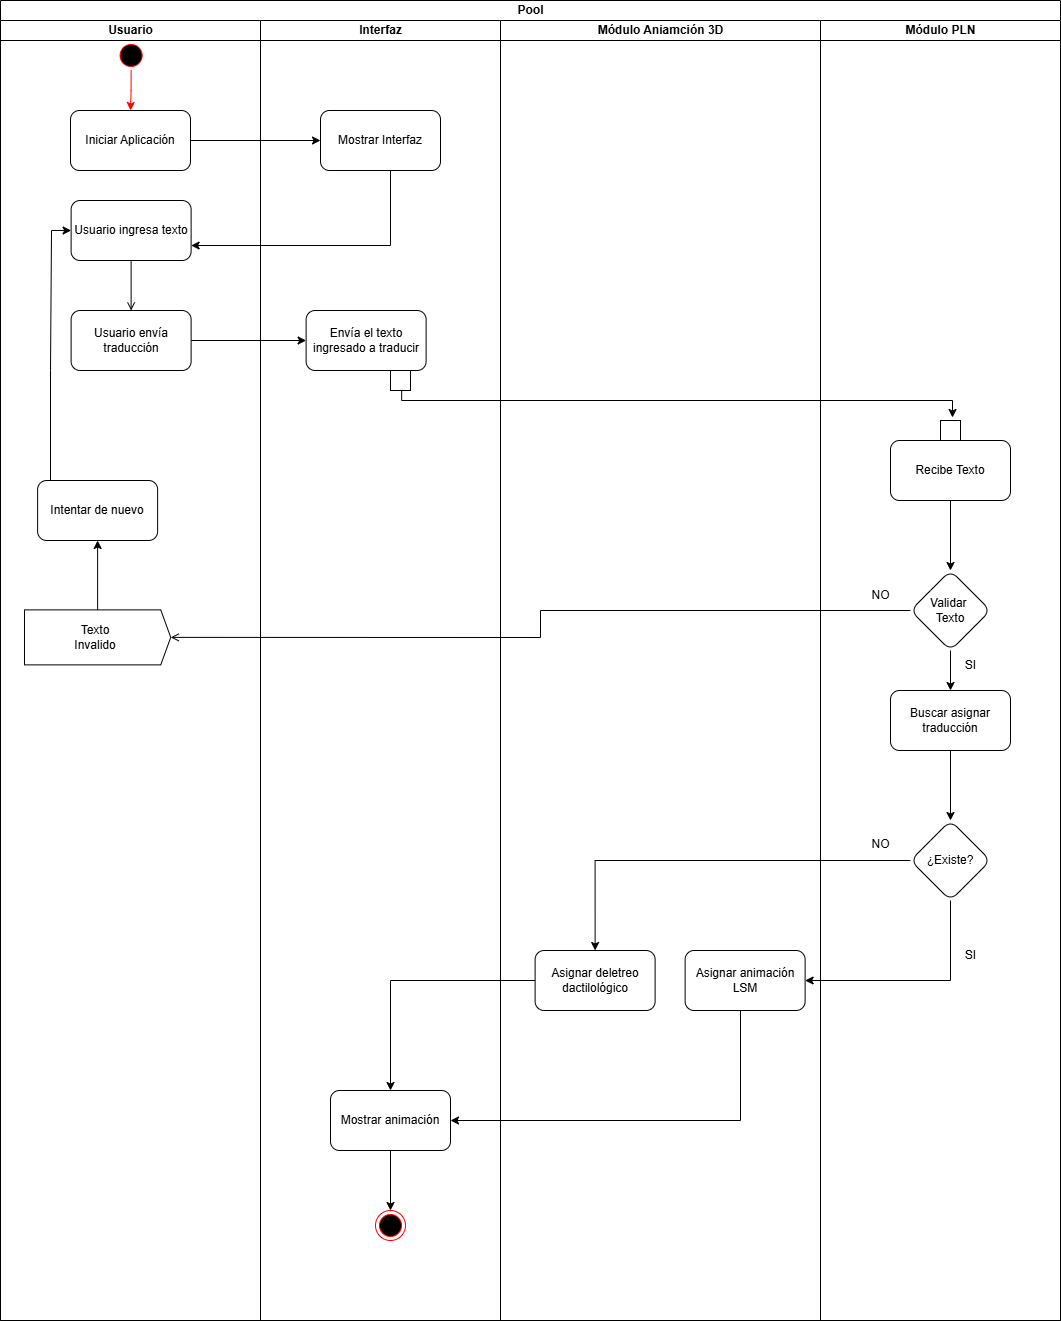
\includegraphics[width=1\textwidth]{Images/Cap 3/Actividades.png}
% 	}
%     \captionof{figure}{Diagrama de actividades del sistema}
% \end{center}

\begin{center}
	\makebox[\textwidth]{%
		\includegraphics[width=1\textwidth]{Images/Cap 2/ProcesoComunicación.png}
	}
    \captionof{figure}[Proceso de comunicación]{Proceso de comunicación, elaboración propia.}
\end{center}

La comunicación es un proceso indispensable para la interacción humana ya que por medio de ella las personas pueden intercambiar ideas, pensamientos y emociones. No obstante, como se menciona en el concepto de ruido, en ocasiones hay elementos que impiden que la comunicación se lleve a cabo, como lo pueden ser las barreras de la comunicación.

\newpage
\subsection{Barreras de la comunicación}
Las barreras de la comunicación son elementos que limitan o dificultan que las personas puedan comunicarse, a la par que se dificulta su proceso de comunicación \cite{ref2}. Son todas las perturbaciones que sufre un mensaje, en cualquiera de los elementos que forman parte del proceso de comunicación.\\

Los principales tipos de barreras son:
\begin{enumerate}
    \item \textbf{Barreras físicas}: son interferencias causadas por elementos del entorno o en el medio donde se lleva a cabo la comunicación \cite{ref25}.
    \item \textbf{Barreras psicológicas}: son aquellas que surgen por emociones, prejuicios o estados mentales que afectan la interpretación del mensaje \cite{ref25}.
    \item \textbf{Barreras semánticas}: surgen cuando hay confusión en el significado de las palabras, debido a una interpretación incorrecta del lenguaje. Generalmente ocurren cuando se habla en un idioma que el emisor o el receptor no entienden, o se emplean conceptos técnicos desconocidos \cite{ref25}.
    \item \textbf{Barreras administrativas}: generalmente se presentan en entornos laborales y son causadas por falta de planeación, malentendidos, falta de claridad en los procesos de comunicación y distorsiones semánticas \cite{ref25}.
    \item \textbf{Barreras culturales}: este tipo de barreras se presentan cuando hay diferencias en costumbres, valores, normas o expresiones entre culturas, que imposibilitan la comunicación \cite{ref25}.
    \item \textbf{Barreras interpersonales}: hace referencia a las barreras en las que hay suposiciones incorrectas y diferentes percepciones \cite{ref25}.
    \item \textbf{Barreras tecnológicas}: fallas y limitaciones que se presentan en medios tecnológicos empleados para la comunicación \cite{ref25}.
    \item \textbf{Barreras fisiológicas}: impedimentos físicos o biológicos causados por deficiencias en los sentidos, enfermedades o condiciones médicas que afectan cualquiera de los sentidos de manera parcial o total, afectando la transmisión de información \cite{ref25}. Por ejemplo, voz débil, pronunciación defectuosa, sordera, problemas del habla, problemas visuales, etc.
\end{enumerate}
Para efectos de este Trabajo Terminal se analizarán las barreras fisiológicas, concretamente las que son causadas por problemas de sordera. En el siguiente apartado se describen los términos correctos para referirse a las personas con capacidad de escucha y a las personas con discapacidad auditiva.\\

\section{Personas con discapacidad auditiva}
\subsection{Personas Oyentes}
Un oyente se define como aquella persona con la capacidad de escuchar sonidos que le permiten interpretar mensajes. El término procede del verbo oír, que refiere a la capacidad que posee un individuo para poder percibir sonidos \cite{ref26}.

\subsection{Personas con discapacidad auditiva (sordas)}
Por otro lado, una persona que padece de discapacidad auditiva es aquella que ha sufrido la pérdida de la función del sistema auditivo, teniendo como consecuencia una discapacidad para poder oír, lo que dificulta el acceso al lenguaje oral \cite{ref27}.\\ 

Los términos adecuados para referirse a las personas que padecen de esta condición son personas sordas, personas con discapacidad auditiva o personas de la comunidad sorda \cite{refsordos}. \\

De acuerdo con la Federación Mundial de Sordos, existen aproximadamente 70 millones de personas sordas en todo el mundo, las cuales emplean más de 300 diferentes lenguas de señas \cite{ref28}. Las lenguas de señas varían entre países, presentando cambios principalmente en la estructura gramatical, sintaxis, vocabulario, signos, alfabeto y expresiones corporales \cite{ref26}.\\

Por otro lado, la Secretaría de Salud menciona que en México hay aproximadamente 2.3 millones de personas con discapacidad auditiva, de las cuales más del 50\% son mayores de 60 años, 34\% tienen entre 30 y 59 años, y el 2\% son niñas y niños \cite{ref3}.\\

Las principales causas de problemas de audición son antecedentes familiares de sordera heredados, edad avanzada, enfermedades infecciosas, exposición continua a sonidos intensos, entre otras \cite{ref3}.\\

Las personas sordas enfrentan consecuencias en ámbitos académicos, laborales, sociales y emocionales, debido a que las situaciones de aislamiento, deficiencia en la comunicación y dificultades del día a día repercuten negativamente para integrarse en grupos y para socializar \cite{ref29}. \\

\newpage
\subsection{Tipos de Discapacidad Auditiva}
La discapacidad auditiva se clasifica en tres tipos según distintos criterios: según la parte del oído afectada, según el grado de pérdida auditiva y según el momento en que se adquiere \cite{ref30}:\\
\newline\textbf{Según la parte del oído afectada}
\begin{itemize}
    \item \textbf{Hipoacusia conductiva}: es producida por un impedimento en el trayecto de las ondas sonoras del oído externo y medio al oído interno, causado por tumores, perforación del tímpano, traumatismos o disfunciones del oído.  
    \item \textbf{Hipoacusia neurosensorial}: se produce cuando el nervio auditivo o las células ciliadas son dañadas, ya sea por herencia, anormalidades al momento del nacimiento, exposición a ruidos fuertes, traumatismos, entre otras causas.  
    \item \textbf{Hipoacusia mixta}: combinación de hipoacusia conductiva e hipoacusia neurosensorial, causadas por anormalidades al nacer, infecciones, tumores y lesiones en la cabeza.  
\end{itemize}

\begin{center}
    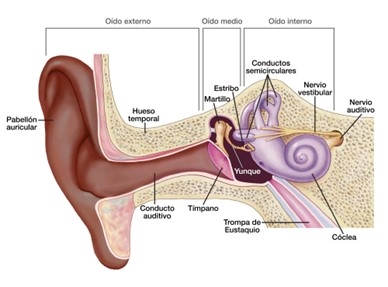
\includegraphics[width=0.9\textwidth]{Images/Cap 2/PartesOido.jpg}
    \captionof{figure}[Partes del oído humano]{Partes del oído humano, obtenido de \cite{ref31}.} 
\end{center}

\newpage
\textbf{Según el grado de pérdida}\\
El rango normal de audición oscila entre 0 y 20 decíbeles (dB). Tomando en consideración ese rango, se establece la siguiente clasificación de acuerdo con los dB que se hayan perdido:

\begin{itemize}
    \item \textbf{Leve:} 20-40 dB.  
    \item \textbf{Moderada:} 40-70 dB.  
    \item \textbf{Severa:} 70-90 dB.  
    \item \textbf{Profunda:} más de 90 dB.  
\end{itemize}

\textbf{Según el momento de la adquisición}\\
En esta clasificación, la discapacidad auditiva puede ser:

\begin{itemize}
    \item \textbf{Hereditaria}: la discapacidad está contenida en algunos de los genes de uno o ambos progenitores.  
    \item \textbf{Adquirida}: la discapacidad puede ser prenatal (antes del nacimiento) o postnatal (después del nacimiento), y en este último caso se deben tomar en cuenta otros criterios:
        \begin{itemize}
        \item \textbf{Prelocutiva:} antes del desarrollo del lenguaje.  
        \item \textbf{Postlocutiva:} después del desarrollo del lenguaje.  
        \end{itemize}
    \end{itemize}

Las personas sordas enfrentan consecuencias en ámbitos académicos, laborales, sociales y emocionales, debido a que las situaciones de aislamiento, deficiencia en la comunicación y dificultades del día a día repercuten negativamente para integrarse en grupos y para socializar \cite{ref29}. En la siguiente sección, se abordan las brechas entre las personas oyentes y las personas con discapacidad.

\subsection{Brechas entre personas oyentes y personas con discapacidad auditiva}
En el plano sociocultural el lenguaje es esencial en las formas de comunicación en una comunidad, pero cuando no todos los individuos pueden responder a esa lógica comunicativa se crean brechas en los discursos que giran en torno a las formas de relacionarse con los demás, puesto que aquellos que tienen códigos y configuraciones diferentes pasan a estar en un plano de invisibilidad \cite{ref32}.\\

La comunidad sorda, a pesar de ser un grupo portador de un lenguaje cultural particular, debe responder a la lengua “natural” de las personas oyentes, y de no poder hacerlo ocasiona que sean excluidos en diferentes escenarios de la vida cotidiana. Esta comunidad ha sido estereotipada como personas incapaces o con limitaciones para insertarse en la sociedad, por lo que, si no pueden entrar en la “lógica natural” para comunicarse con las personas, se ven forzados a interactuar solamente con las personas que comparten su misma condición \cite{ref32}.\\

A lo largo de los últimos años, se han realizado múltiples esfuerzos a nivel gubernamental y se han puesto en marcha discursos que giran alrededor del reconocimiento e inclusión de todas las personas por igual, como lo es la Ley General para la Inclusión de las Personas con Discapacidad \cite{ref37}, para garantizar una mayor participación de las personas con discapacidad auditiva en escenarios sociales. No obstante, lo expresado en la legalidad dista mucho de las realidades particulares de las personas sordas en el marco sociocultural. La comunidad sorda ha sido reconocida como minoría lingüística y, por sus mismas condiciones, ha sido ubicada socialmente en el plano de la exclusión y la invisibilidad \cite{ref32}. \\ 

La presencia de barreras de comunicación generan aislamiento e impiden el desarrollo de una existencia satisfactoria, lo que puede generar graves problemas psicológicos como la depresión, ansiedad, insomnio, estrés, ideas paranoides y sensibilidad interpersonal \cite{ref27}.\\

Además, la comunidad sorda presenta dificultad para acceder a la información proveniente de la televisión, radio, llamadas telefónicas, megafonías en estaciones de metro y salidas de aeropuertos, etc., debido a que esta es principalmente transmitida hacia la población oyente.\\

A pesar de que las personas sordas presentan muchas dificultades en su vida diaria, hoy en día disponen de numerosas herramientas de apoyo (ver \autoref{sec:edoArte}) para impulsar su inclusión en entornos sociales y favorecer su crecimiento personal, como lo son las prótesis auditivas, señales acústicas y su propia Lengua de Señas. \\

En este Trabajo Terminal, únicamente se centrará el estudio en las Lenguas de Señas, concretamente en la Lengua de Señas Mexicana (LSM), revisando toda la documentación existente hasta el 2024, año de la elaboración de este trabajo.\\

\newpage
\section{Lengua de Señas Mexicana}
\subsection{Definición de Lengua de Señas}
La Lengua de Señas es definida como la lengua natural de expresión y configuración gesto-espacial y percepción visual gracias a la cual los sordos pueden comunicarse con su entorno social, la cual está basada en movimientos y expresiones a través de manos, ojos, rostro, boca y cuerpo \cite{ref33}.\\

En el mundo existen cerca de 300 lenguas de señas distintas, siendo así que cada país posee su propia lengua de señas. Por ejemplo, la Lengua de Señas Mexicana (LSM) es diferente a la Lengua de Señas Española (LSE), que a pesar de estar articulados en el mismo idioma (español), no comparten muchas señas en común debido a que ambas lenguas presentan señas que pueden ser regionalismos de cada país \cite{ref33}.\\

Por su parte, la Lengua de Señas Mexicana (LSM) es la lengua de señas que se emplea en México, que cuenta con su propio vocabulario y gramática. A la LSM se le considera como una lengua, debido a que es completamente capaz de expresar una amplia gama de pensamientos y emociones como cualquier otra lengua \cite{ref33}.

\subsection{Lengua de Señas Mexicana (LSM)}
La Ley General para la Inclusión de las Personas con Discapacidad \cite{ref34} define a la LSM, en el Artículo 2, como la lengua de una comunidad de sordos que consiste en una serie de signos gestuales articulados con las manos y acompañados de expresiones faciales, mirada intencional y movimiento corporal, dotados de función lingüística, que forma parte del patrimonio lingüistico de dicha comunidad y es tan rica y compleja en gramática y vocabulario como cualquier lengua oral \cite{ref34}.\\

Por su parte, el Artículo 20 de dicha ley establece que los medios de comunicación deben implementar la tecnología, más concretamente, de intérpretes de LSM que permitan a la comunidad de sordos las facilidades de comunicación \cite{ref34}.\\

En México hay entre 87,000 y 100,000 personas hablantes de LSM que la dominan y la emplean como vía de comunicación, siendo incluso una población mucho más grande que algunas comunidades hablantes de lenguas indígenas del país \cite{ref35}.\\

\newpage
\subsection{Abecedario de la LSM}
La siguiente tabla explica detalladamente cómo se conforma cada una de las letras del abecedario de LSM:

\begin{longtable}{|m{2cm}|m{5cm}|m{5cm}|}
    \hline
    \textbf{Letra} & \textbf{Descripción} & \textbf{Seña} \\
    \hline
    \endfirsthead
    
    \hline
    \textbf{Letra} & \textbf{Descripción} & \textbf{Seña} \\
    \hline
    \endhead
    
    \hline
    \endfoot
    
    \endlastfoot
    
    A & Con la mano cerrada, se muestran las uñas y se estira el dedo pulgar hacia un lado. La palma mira al frente.
    & \makecell{\colorbox{white}{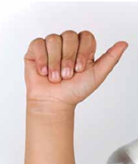
\includegraphics[width=4cm]{Images/Cap 2/Alfabeto LSM/A.png}}} \\
    \hline
    
    B & Los dedos índice, medio, anular y meñique se estiran unidos y el pulgar se dobla hacia la palma, la cual mira al frente.
    & \makecell{\colorbox{white}{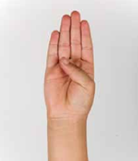
\includegraphics[width=4cm]{Images/Cap 2/Alfabeto LSM/B.png}}} \\
    \hline
    
    C & Los dedos índice, medio, anular y meñique se mantienen unidos y en posición cóncava; el pulgar también se coloca en esa posición. La palma mira a un lado.
    & \makecell{\colorbox{white}{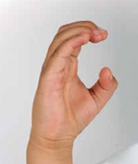
\includegraphics[width=4cm]{Images/Cap 2/Alfabeto LSM/C.png}}} \\
    \hline

    D & Los dedos medio, anular, meñique y pulgar se unen por las puntas y el dedo índice se estira. La palma mira al frente.
    & \makecell{\colorbox{white}{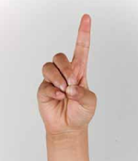
\includegraphics[width=4cm]{Images/Cap 2/Alfabeto LSM/D.png}}} \\
    \hline

    E & Se doblan los dedos completamente y se muestran las uñas. La palma mira al frente.
    & \makecell{\colorbox{white}{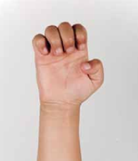
\includegraphics[width=4cm]{Images/Cap 2/Alfabeto LSM/E.png}}} \\
    \hline

    F & Con la mano abierta y los dedos unidos, se dobla el índice hasta que su parte lateral toque la yema del pulgar. La palma mira a un lado.
    & \makecell{\colorbox{white}{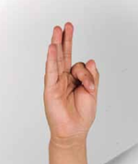
\includegraphics[width=4cm]{Images/Cap 2/Alfabeto LSM/F.png}}} \\
    \hline

    G & Se cierra la mano y los dedos índice y pulgar se estiran. La palma mira hacia la persona que se comunica.
    & \makecell{\colorbox{white}{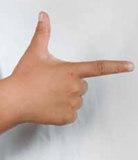
\includegraphics[width=4cm]{Images/Cap 2/Alfabeto LSM/G.png}}} \\
    \hline

    H & Se cierra la mano y los dedos índice y medio se unen y se estiran, se extiende el dedo pulgar señalando hacia arriba. La palma mira hacia la persona que se comunica.
    & \makecell{\colorbox{white}{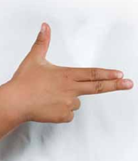
\includegraphics[width=4cm]{Images/Cap 2/Alfabeto LSM/H.png}}} \\
    \hline

    I & Con la mano cerrada, el dedo meñique se estira señalando hacia arriba. La palma se coloca de lado.
    & \makecell{\colorbox{white}{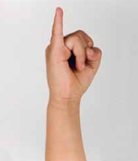
\includegraphics[width=4cm]{Images/Cap 2/Alfabeto LSM/I.png}}} \\
    \hline

    J & Con la mano cerrada, el dedo meñique estirado señala hacia arriba y la palma señala a un lado. La mano dibuja una “j” en el aire.
    & \makecell{\colorbox{white}{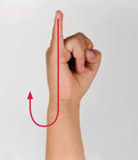
\includegraphics[width=4cm]{Images/Cap 2/Alfabeto LSM/J.png}}} \\
    \hline

    K & Se cierra la mano con los dedos índice, medio y pulgar estirados. La yema del pulgar se coloca entre el índice y el medio, moviendo la muñeca hacia arriba.
    & \makecell{\colorbox{white}{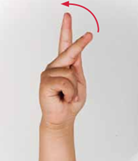
\includegraphics[width=4cm]{Images/Cap 2/Alfabeto LSM/K.png}}} \\
    \hline

    L & Con la mano cerrada y los dedos índice y pulgar estiados, se forma una “L”. La palma mira al frente.
    & \makecell{\colorbox{white}{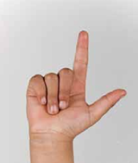
\includegraphics[width=4cm]{Images/Cap 2/Alfabeto LSM/L.png}}} \\
    \hline

    M & Con la mano cerrada, se ponen los dedos índice, medio y anular sobre el pulgar.
    & \makecell{\colorbox{white}{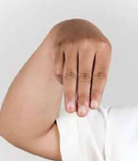
\includegraphics[width=4cm]{Images/Cap 2/Alfabeto LSM/M.png}}} \\
    \hline
 
    N & Con la mano cerrada, se ponen los dedos índice y medio sobre el pulgar. 
    & \makecell{\colorbox{white}{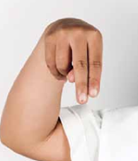
\includegraphics[width=4cm]{Images/Cap 2/Alfabeto LSM/N.png}}} \\
    \hline

    Ñ & Con la mano cerrada, se ponen los dedos índice y medio sobre el pulgar. Se mueve la muñeca a los lados. 
    & \makecell{\colorbox{white}{\includegraphics[width=4cm]{Images/Cap 2/Alfabeto LSM/Ñ.png}}} \\
    \hline

    O & Con la mano se forma una letra “o”. Todos los dedos se tocan por las puntas. 
    & \makecell{\colorbox{white}{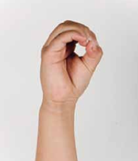
\includegraphics[width=4cm]{Images/Cap 2/Alfabeto LSM/O.png}}} \\
    \hline

    P & Con la mano cerrada y los dedos índice, medio y pulgar estirados, se coloca la yema del pulgar entre el índice y el medio.
    & \makecell{\colorbox{white}{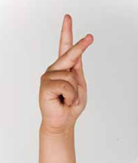
\includegraphics[width=4cm]{Images/Cap 2/Alfabeto LSM/P.png}}} \\
    \hline
    
    Q & Con la mano cerrada, se colocan los dedos índice y pulgar en posición de garra. La palma mira hacia abajo, y se mueve hacia los lados.
    & \makecell{\colorbox{white}{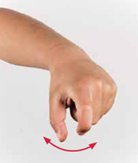
\includegraphics[width=4cm]{Images/Cap 2/Alfabeto LSM/Q.png}}} \\
    \hline
    
    R & Con la mano cerrada, se estiran y entrelazan los dedos índice y medio. La palma mira al frente.
    & \makecell{\colorbox{white}{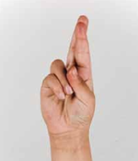
\includegraphics[width=4cm]{Images/Cap 2/Alfabeto LSM/R.png}}} \\
    \hline

    S & Con la mano cerrada, se pone el pulgar sobre los otros dedos. La palma mira al frente.
    & \makecell{\colorbox{white}{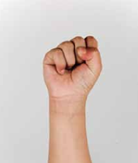
\includegraphics[width=4cm]{Images/Cap 2/Alfabeto LSM/S.png}}} \\
    \hline

    T & Con la mano cerrada, el pulgar se pone entre el índice y el medio. La palma mira al frente. 
    & \makecell{\colorbox{white}{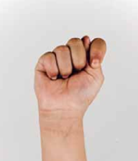
\includegraphics[width=4cm]{Images/Cap 2/Alfabeto LSM/T.png}}} \\
    \hline

    U & Con la mano cerrada, se estiran los dedos índice y medio unidos. La palma mira al frente. 
    & \makecell{\colorbox{white}{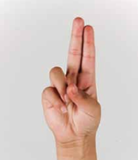
\includegraphics[width=4cm]{Images/Cap 2/Alfabeto LSM/U.png}}} \\
    \hline

    V & Con la mano cerrada, se estiran los dedos índice y medio separados. La palma mira al frente. 
    & \makecell{\colorbox{white}{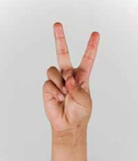
\includegraphics[width=4cm]{Images/Cap 2/Alfabeto LSM/V.png}}} \\
    \hline

    W & Con la mano cerrada, se estiran los dedos índice, medio y anular separados. La palma mira al frente. 
    & \makecell{\colorbox{white}{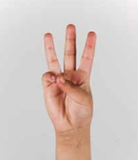
\includegraphics[width=4cm]{Images/Cap 2/Alfabeto LSM/W.png}}} \\
    \hline

    X & Con la mano cerrada, el índice y el pulgar en posición de garra y la palma dirigida a un lado, se realiza un movimiento al frente y de regreso. 
    & \makecell{\colorbox{white}{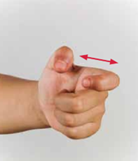
\includegraphics[width=4cm]{Images/Cap 2/Alfabeto LSM/X.png}}} \\
    \hline
    
    Y & Con la mano cerrada, se estira el meñique y el pulgar. La palma mira hacia la persona que se comunica. 
    & \makecell{\colorbox{white}{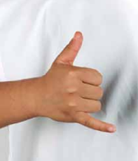
\includegraphics[width=4cm]{Images/Cap 2/Alfabeto LSM/Y.png}}} \\
    \hline

    Z & Con la mano cerrada, el dedo índice estirado y la palma al frente, se dibuja una letra z en el aire. 
    & \makecell{\colorbox{white}{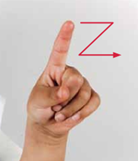
\includegraphics[width=4cm]{Images/Cap 2/Alfabeto LSM/Z.png}}} \\
    \hline
    
    \caption[Abecedario de la LSM]{Abecedario de la LSM, obtenido de \cite{ref36}.} \label{tabla:LSM}
\end{longtable}

\clearpage

\subsection{Grámatica de la Lengua de Señas Mexicana}
La gramática estudia cómo se conectan los elementos de una lengua para crear oraciones con sentido. En la Lengua de Señas Mexicana (LSM), esa estructura no depende de sonidos ni palabras habladas, sino del uso visual del cuerpo, el espacio y los movimientos \cite{ref37}.\\

La LSM se desarrolla en un espacio frente al cuerpo, dividido en tres zonas principales \cite{ref37}:

\begin{itemize}
    \item Una línea vertical que va desde la cintura hasta la parte superior de la cabeza.
    \item Un límite horizontal, que se extiende hasta los codos con los brazos en ángulo.
    \item Un tercer límite que marca qué tan lejos están las manos del cuerpo.
\end{itemize}

Si la seña se realiza fuera de estos límites, suele entenderse como un énfasis o exageración del mensaje.\\

A diferencia del español, la LSM no se basa en sonidos, sino en aspectos visuales y espaciales. Las señas suelen representar ideas complejas, como si fueran palabras individuales con sentido propio. Estas señas se consideran morfemas libres, ya que no necesitan agregarse a otras ni modificarse con terminaciones \cite{ref38}.\\

En esta lengua, no se usan frecuentemente sufijos y prefijos para cambiar el significado. En su lugar, expresiones faciales, movimientos de cabeza o del cuerpo ayudan a matizar lo que se dice. Estos gestos pueden aportar información como si la acción se repite, si está terminada, si es deseada, obligatoria, o si es posible \cite{ref38}.\\

Las señas no tienen una categoría gramatical fija. Una misma seña puede funcionar como verbo, adjetivo o sustantivo, dependiendo del contexto en que se use. Esta flexibilidad se debe a un fenómeno llamado prototipicidad, que permite a ciertas formas adaptarse a distintas funciones según la necesidad \cite{ref38}.\\

Existen señas que siguen patrones más estables, como los verbos direccionales, que cambian su movimiento para indicar quién realiza una acción y hacia quién va dirigida. Sin embargo, estas señas también pueden usarse en otros contextos sin perder su significado \cite{ref38}.\\

Las oraciones en LSM se forman con señas que expresan acciones, participantes, tiempo, condiciones o características. En oraciones simples, las señas que representan sujetos u objetos se comportan como nombres, aunque no siempre sean sustantivos. Las acciones o ideas principales se representan con señas que funcionan como predicados \cite{ref38}.\\

También es común ver señas que expresan pronombres, ubicaciones o tiempos. A veces se usa el deletreo dactilológico o nombres propios, los cuales pueden repetirse al final de la oración como una forma de remarcar la información, lo que algunos estudios llaman “etiquetado” o “tags” \cite{ref38}.\\

\begin{center}
    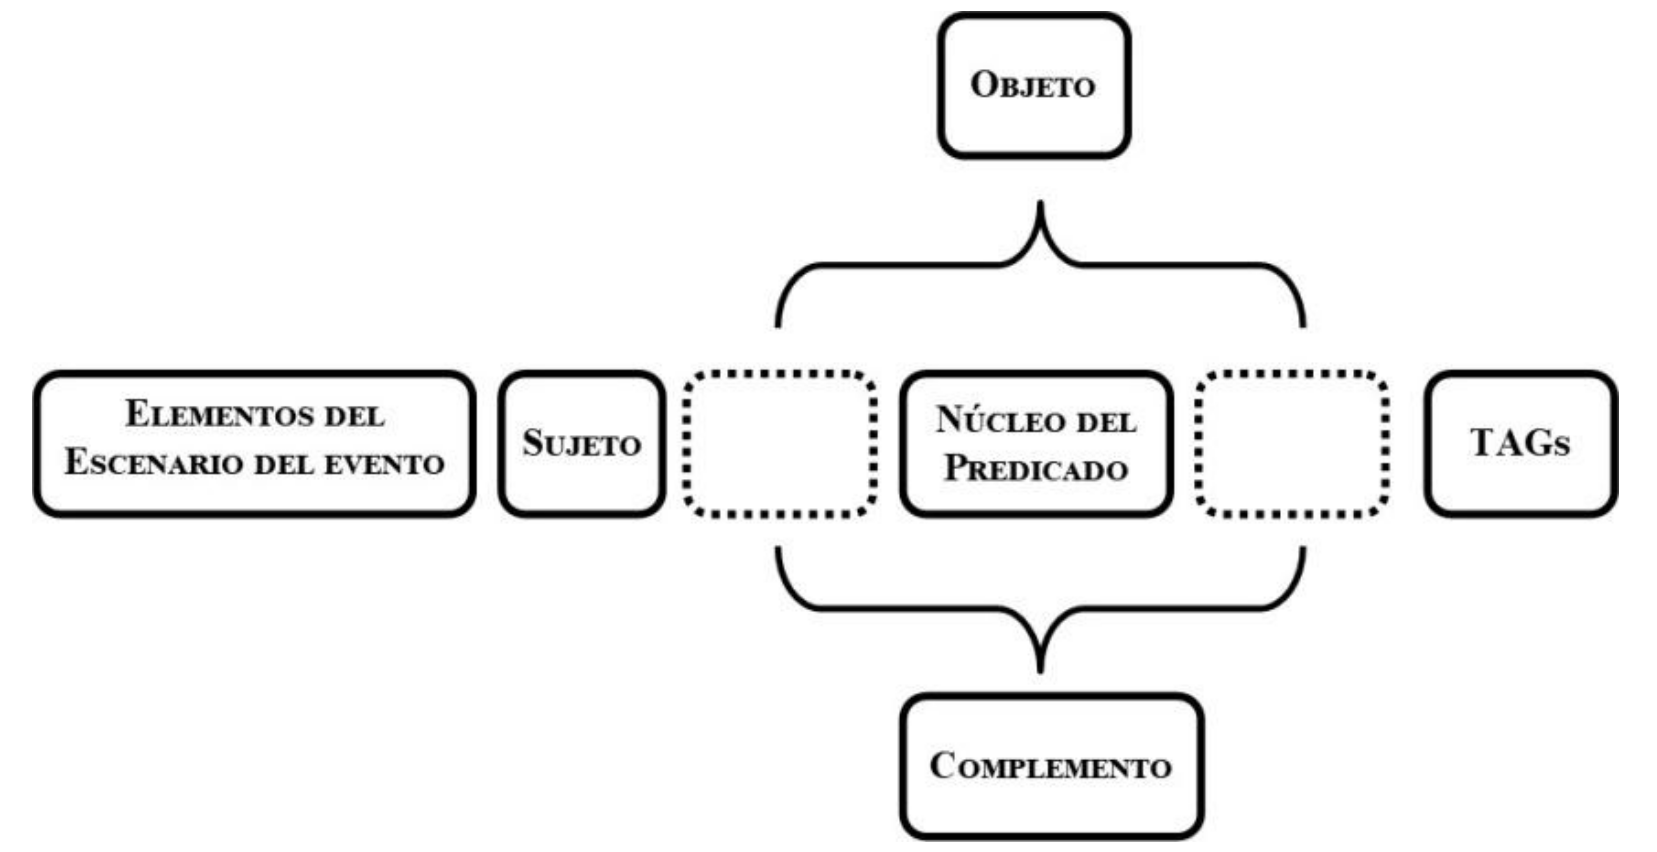
\includegraphics[width=0.9\textwidth]{Images/Cap 2/Estructura_gramatica_LSM.png}
    \captionof{figure}[Estructura gramatical de una oración de LSM]{Estructura gramatical de una oración de LSM, obtenido de \cite{ref38}.}  % Pie de foto manual
\end{center}

\textbf{Fonología}\\
En las lenguas de señas, los fonemas, las unidades mínimas con significado, pueden descomponerse en siete componentes esenciales \cite{ref39}:

\begin{enumerate}
    \item \textbf{Configuración manual}: es la forma específica que adopta la mano al ejecutar un signo determinado.
    \item \textbf{Orientación de la mano}: hace referencia a la dirección en la que se posiciona la palma, ya sea orientada hacia arriba, abajo o frente al emisor.
    \item \textbf{Zona de ejecución}: indica la parte del cuerpo en la que se realiza el signo, como por ejemplo la frente, la boca, el pecho o los hombros.
    \item \textbf{Desplazamiento}: describe el tipo de movimiento que se lleva a cabo con las manos al hacer un signo; este puede ser giratorio, lineal, en vaivén o segmentado.
    \item \textbf{Área de contacto}: se refiere a la parte de la mano dominante (la derecha para personas diestras o la izquierda para personas zurdas) que entra en contacto con el cuerpo. Puede involucrar la palma, las yemas o el dorso de los dedos.
    \item \textbf{Plano de producción}: se trata de la distancia entre el cuerpo y el lugar donde se articula el signo. El Plano 1 está en contacto directo con el cuerpo, mientras que el Plano 4 se encuentra más alejado, con los brazos completamente extendidos.
    \item \textbf{Elementos corporales no manuales}: son señales complementarias que refuerzan el mensaje, como expresiones faciales, movimientos del torso, gesticulaciones orales o el uso del cuello y los hombros. Por ejemplo, para comunicar una acción futura se inclina el cuerpo hacia delante, y para indicar el pasado, hacia atrás.\\
\end{enumerate}

\textbf{La Configuración Manual (CM) en la LSM}\\
\label{sec:config_manual}
En las lenguas de señas, las manos son las principales herramientas para comunicar, aunque no son las únicas. Además de considerar la dirección del movimiento y el lugar en el espacio donde se hace una seña, también es esencial observar la forma que toman las manos, conocida como configuración manual (CM). Esta configuración puede variar tanto en la mano dominante como en la no dominante \cite{ref37}.\\

La configuración manual, entonces, representa la forma específica que adoptan las manos al momento de hacer una seña. Esto incluye aspectos como \cite{ref37}:

\begin{itemize}
    \item \textbf{La posición de los dedos}: si están juntos o separados, doblados o rectos.
    \item \textbf{La forma general de la mano}: abierta, en puño, en forma de garra, etc.
    \item \textbf{La ubicación del pulgar y del índice}: suelen tener movimientos propios.
\end{itemize}

Desde un punto de vista técnico, la configuración manual forma parte de lo que se llama la matriz articulatoria. Dentro de ella, se distinguen dos grupos importantes \cite{ref37}:

\begin{itemize}
    \item Los dedos (índice, medio, anular y meñique), que suelen moverse como bloque.
    \item El pulgar, que, por su movilidad más independiente, se analiza aparte.
\end{itemize}

Debido a todas las combinaciones posibles entre estos elementos, las configuraciones manuales no pueden reducirse a formas simples, sino que son estructuras complejas que generan significado cuando se combinan con otros componentes de la seña.

\newpage

\textbf{Orientación de la Palma de la Mano}\\
Se refiere a la dirección en la que se encuentra la palma de la mano en relación con el cuerpo de la persona que está haciendo la seña, justo en el momento en que adopta la configuración manual \cite{ref37}.\\

En la Lengua de Señas Mexicana (LSM), se han identificado nueve posibles formas de orientar la palma durante la articulación de una seña \cite{ref37}. Estas son:

\begin{enumerate}
    \item Palma hacia arriba, con los dedos apuntando a la izquierda.
    \item Palma hacia arriba, con los dedos apuntando hacia el frente.
    \item Palma hacia abajo, con los dedos dirigidos a la izquierda.
    \item Palma hacia abajo, con los dedos apuntando hacia adelante.
    \item Palma hacia la izquierda, con los dedos hacia arriba.
    \item Palma hacia la izquierda, con los dedos hacia el frente.
    \item Palma hacia el frente, con los dedos señalando hacia arriba.
    \item Palma frente al cuerpo, dedos hacia arriba.
    \item Palma frente al cuerpo, dedos hacia la izquierda.
\end{enumerate}

\begin{center}
    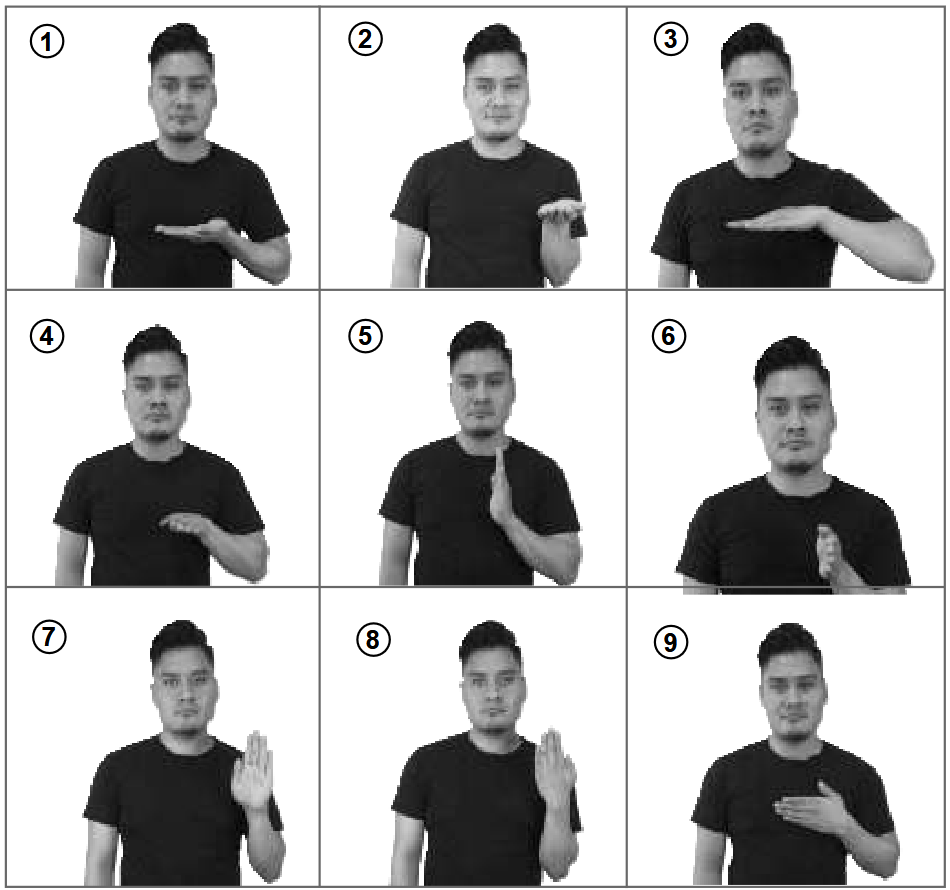
\includegraphics[width=0.7\textwidth]{Images/Cap 2/Orientacion_Palma_Mano.png}
    \captionof{figure}[Orientaciones de la palma de la mano en LSM]{Orientaciones de la palma de la mano en LSM, obtenido de \cite{ref37}.}  % Pie de foto manual
\end{center}

Cada una de estas orientaciones forma parte de la estructura visual y espacial de una seña, y su correcta ejecución es clave para transmitir el significado deseado.\\

\textbf{Ubicación en la Lengua de Señas Mexicana (LSM)}\\
Hace referencia al lugar específico en el espacio donde se realiza una seña. Este espacio, conocido como espacio señante, puede estar frente al cuerpo o sobre él y es clave para transmitir el significado correcto \cite{ref37}.\\

Para describir las señas en este diccionario, se dividió el espacio señante principalmente en niveles de altura y direcciones laterales. En algunos casos, también se toma en cuenta una tercera dimensión, que implica mayor cercanía o profundidad \cite{ref37}.\\

Cuando las señas se hacen sobre el cuerpo, se habla de “alturas” específicas, como por ejemplo:
\begin{itemize}
    \item A la altura del cuello.
    \item A la altura del hombro.
    \item A la altura del pecho.
    \item A la altura del plexo.
    \item A la altura de la cintura.
    \item A la altura de la cadera.
\end{itemize}

Si la seña se mueve entre dos puntos, se describe como un desplazamiento, por ejemplo:

\begin{itemize}
    \item Del pecho a la cintura.
    \item Del hombro a la cadera.
    \item Del cuello a la cadera.
\end{itemize}

Cuando el movimiento es horizontal o de un lado a otro, también se aclara, por ejemplo:
\begin{itemize}
    \item A la altura del pecho, de izquierda a derecha.
\end{itemize}

En el caso de las señas realizadas en la cara, se puede ser más preciso indicando zonas como:
\begin{itemize}
    \item A la altura de los ojos.
    \item A la altura de las cejas.    
\end{itemize}

Finalmente, si la seña se hace sobre el tronco del cuerpo, se especifica si es:
\begin{itemize}
    \item Del lado izquierdo.
    \item Del lado derecho.
    \item Al centro.
\end{itemize}

Aunque algunas ubicaciones pueden detallarse aún más, se busca usar una descripción unificada para facilitar la comprensión \cite{ref37}.\\

\textbf{Dirección del Movimiento de la mano en la LSM}\\
Es la trayectoria que la mano sigue al realizar una seña \cite{ref37}. En la \autoref{direcciones_Mano} se muestran las nueve direcciones que las configuraciones manuales pueden seguir durante la articulación de las señas respecto al cuerpo.

\begin{center}
    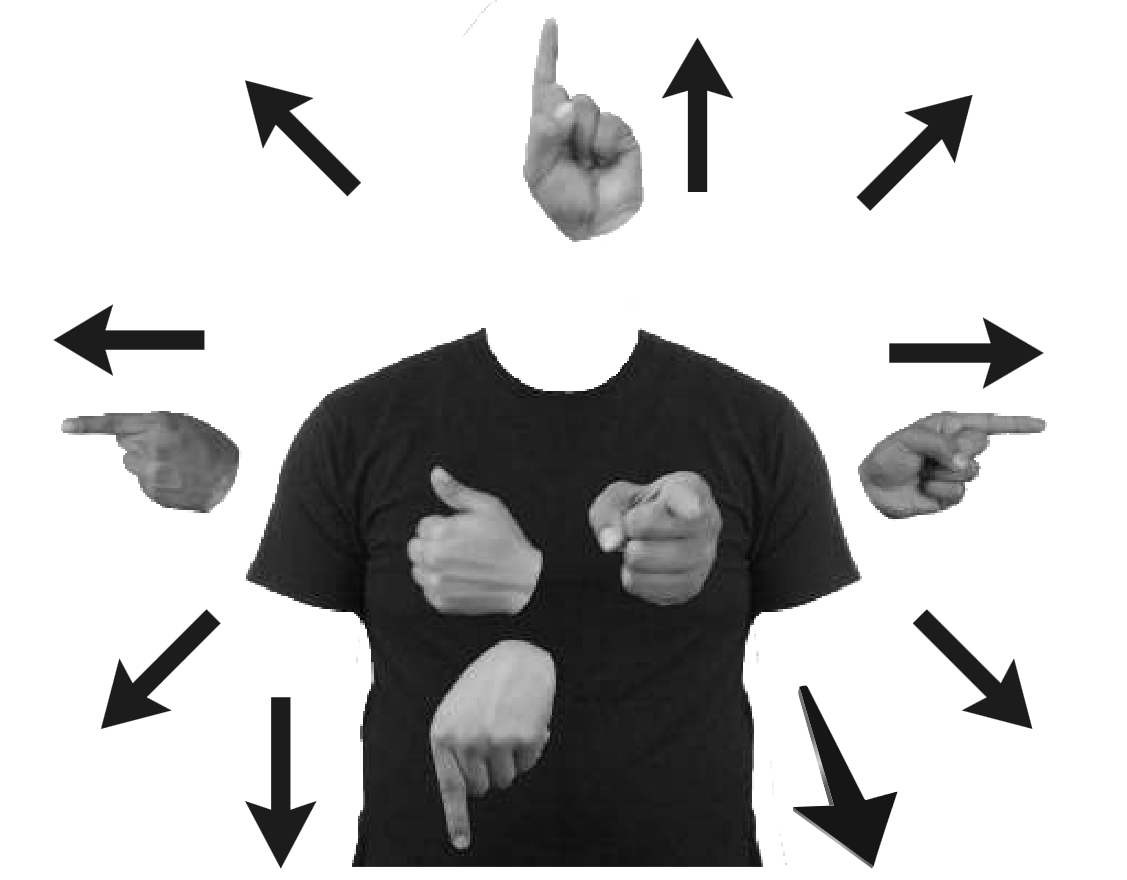
\includegraphics[width=0.8\textwidth]{Images/Cap 2/Direccion_Manos_LSM.png}
    \captionof{figure}[Direcciones posibles que sigue la mano en la LSM]{Direcciones posibles que sigue la mano en la LSM, obtenido de \cite{ref37}.} 
    \label{direcciones_Mano}
\end{center}

\newpage
\textbf{Explicación de los movimientos y sus símbolos}\\
La \autoref{tabla:Movimiento_LSM} muestra todos los movimientos que las manos pueden realizar en la LSM. En la primera columna se menciona el nombre del movimiento; en la segunda, la descripción del mismo y en la tercera aparecen flechas o imágenes de la mano para indicar la dirección o la manera en que las configuraciones manuales se mueven.\\

\begin{longtable}{|m{5cm}|m{5cm}|m{5cm}|}
    \hline
    \textbf{Movimiento} & \textbf{Descripción del movimiento} & \textbf{Imagen} \\
    \hline
    \endfirsthead
    
    \hline
    \textbf{Movimiento} & \textbf{Descripción del movimiento} & \textbf{Imagen} \\
    \hline
    \endhead
    
    \hline
    \endfoot
    
    \endlastfoot
    
     & Se emplea una numeración progresiva para señalar cómo cambian las formas de las manos y los desplazamientos en las señas que combinan varios movimientos.
    & \makecell{\colorbox{white}{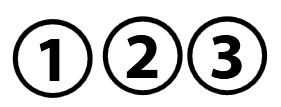
\includegraphics[width=4cm]{Images/Cap 2/Movimientos LSM/1.png}}} \\
    \hline

    Lineal (lin) & Movimiento rectilíneo.
    & \makecell{\colorbox{white}{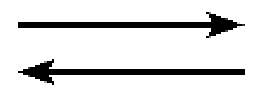
\includegraphics[width=4cm]{Images/Cap 2/Movimientos LSM/2.png}}} \\
    \hline

    Arco (ar) & El desplazamiento del brazo, la muñeca o la mano dibuja una curva en forma de arco.
    & \makecell{\colorbox{white}{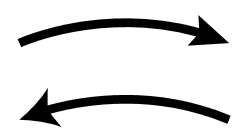
\includegraphics[width=4cm]{Images/Cap 2/Movimientos LSM/3.png}}} \\
    \hline

    Extensión de dedos (E) & Los dedos se extienden.
    & \makecell{\colorbox{white}{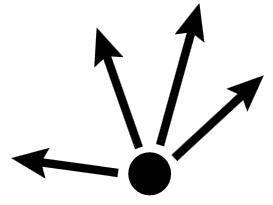
\includegraphics[width=4cm]{Images/Cap 2/Movimientos LSM/4.png}}} \\
    \hline

    Vaivén (va) & Se realiza un movimiento intercalado entre ambas manos o brazos.
    & \makecell{\colorbox{white}{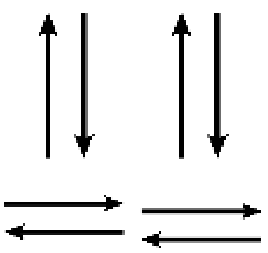
\includegraphics[width=4cm]{Images/Cap 2/Movimientos LSM/5.png}}} \\
    \hline
    
    Circular (circ) & La trayectoria de la mano, muñeca o brazo describe movimientos circulares o semicirculares.
    & \makecell{\colorbox{white}{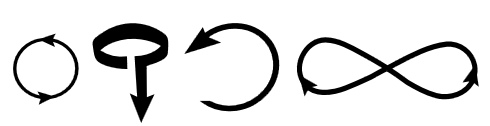
\includegraphics[width=4cm]{Images/Cap 2/Movimientos LSM/6.png}}} \\
    \hline

    Espiral (es) & La mano o el brazo giran siguiendo un patrón redondeado.
    & \makecell{\colorbox{white}{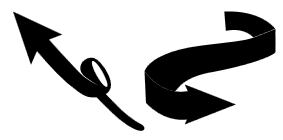
\includegraphics[width=4cm]{Images/Cap 2/Movimientos LSM/7.png}}} \\
    \hline

    Flexión de dedos (f) & Los dedos se retraen.
    & \makecell{\colorbox{white}{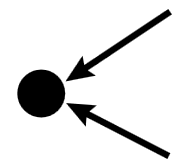
\includegraphics[width=4cm]{Images/Cap 2/Movimientos LSM/8.png}}} \\
    \hline

    Ondular (ond) & El movimiento de la mano o el brazo imita una forma de onda.
    & \makecell{\colorbox{white}{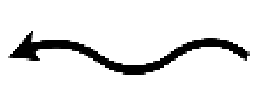
\includegraphics[width=4cm]{Images/Cap 2/Movimientos LSM/9.png}}} \\
    \hline
    
    Salto & La mano o los dedos simulan uno o varios saltos.
    & \makecell{\colorbox{white}{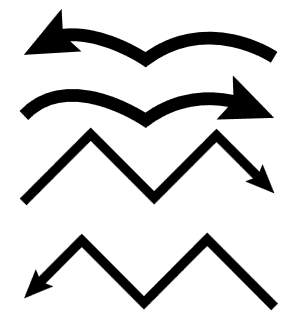
\includegraphics[width=4cm]{Images/Cap 2/Movimientos LSM/10.png}}} \\
    \hline

    Movimiento vibratorio local (vib) & La mano tiembla.
    & \makecell{\colorbox{white}{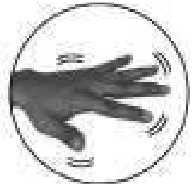
\includegraphics[width=4cm]{Images/Cap 2/Movimientos LSM/11.png}}} \\
    \hline
    
    Cabeceo de muñeca (cab) & El movimiento parte desde la parte posterior y avanza al frente, usando solo el giro de la muñeca.
    & \makecell{\colorbox{white}{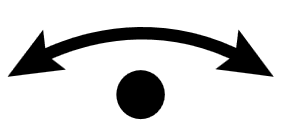
\includegraphics[width=4cm]{Images/Cap 2/Movimientos LSM/12.png}}} \\
    \hline
    
    Aplanado (apl) & Se realiza un contacto breve entre el índice y medio, o el índice y el pulgar, seguido de una separación.
    & \makecell{\colorbox{white}{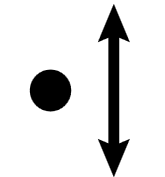
\includegraphics[width=4cm]{Images/Cap 2/Movimientos LSM/13.png}}} \\
    \hline

    Apulgarado (p) & El índice o medio se libera con impulso del pulgar, pasando de estar doblado a completamente recto.
    & \makecell{\colorbox{white}{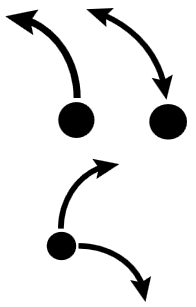
\includegraphics[width=4cm]{Images/Cap 2/Movimientos LSM/14.png}}} \\
    \hline

    Cambios progresivos en los dedos (prog) & Los dedos se mueven uno a uno de forma intercalada.
    & \makecell{\colorbox{white}{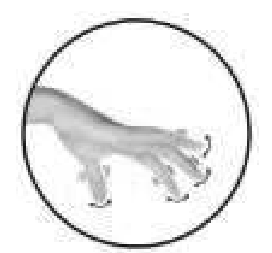
\includegraphics[width=4cm]{Images/Cap 2/Movimientos LSM/15.png}}} \\
    \hline

    Deslizamiento (desl) & Se realiza un movimiento deslizante de los dedos sobre la superficie del pulgar.
    & \makecell{\colorbox{white}{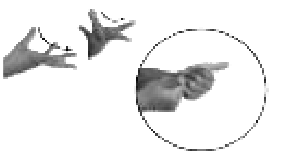
\includegraphics[width=4cm]{Images/Cap 2/Movimientos LSM/16.png}}} \\
    \hline

    Zig-zag (zig) & El índice traza en el aire la forma de la letra Z.
    & \makecell{\colorbox{white}{\includegraphics[width=4cm]{Images/Cap 2/Movimientos LSM/17.png}}} \\
    \hline
    
    Siete (7) & Se realiza un movimiento que dibuja el número siete en el espacio.
    & \makecell{\colorbox{white}{\includegraphics[width=4cm]{Images/Cap 2/Movimientos LSM/18.png}}} \\
    \hline

    Rotación de muñeca (rot) & La rotación del antebrazo o la muñeca provoca que la mano cambie su dirección.
    & \makecell{\colorbox{white}{\includegraphics[width=4cm]{Images/Cap 2/Movimientos LSM/19.png}}} \\
    \hline
    
    Choque (ch) & Las manos se encuentran y se tocan.
    & \makecell{\colorbox{white}{\includegraphics[width=4cm]{Images/Cap 2/Movimientos LSM/20.png}}} \\
    \hline
    
    Doblar (dob) & Mientras el pulgar permanece quieto, los demás dedos se doblan hacia el centro de la mano.
    & \makecell{\colorbox{white}{\includegraphics[width=4cm]{Images/Cap 2/Movimientos LSM/21.png}}} \\
    \hline
    
    Cruzado (crz) & Los brazos se mueven hacia el centro cruzándose, y las manos se aproximan en un punto medio.
    & \makecell{\colorbox{white}{\includegraphics[width=4cm]{Images/Cap 2/Movimientos LSM/22.png}}} \\
    \hline
    
    Simétrico (sim) & Desde una posición inicial común, las manos se separan hacia diferentes direcciones: superior, inferior o lateral.
    & \makecell{\colorbox{white}{\includegraphics[width=4cm]{Images/Cap 2/Movimientos LSM/23.png}}} \\
    \hline

    Prensar & El índice y el pulgar realizan un gesto de pinza al agarrar otra mano o una zona del cuerpo.
    & \makecell{\colorbox{white}{\includegraphics[width=4cm]{Images/Cap 2/Movimientos LSM/24.png}}} \\
    \hline

    \caption[Movimientos de las manos]{Movimientos de las manos, obtenido de \cite{ref37}.} \label{tabla:Movimiento_LSM} \\
\end{longtable}

\textbf{Rasgos no manuales: expresión facial y gestos}\\
Los rasgos no manuales (RNM) en la Lengua de Señas Mexicana incluyen la expresión facial, los gestos y los movimientos del cuerpo \cite{ref37}. Estos elementos se realizan al mismo tiempo que las señas y tienen una función gramatical clave, ya que aportan significado al mensaje, similar a cómo el tono de voz o la velocidad lo hacen en el español hablado \cite{ref37}.\\

También existen gestos universales que no dependen del idioma o la cultura, como los que expresan felicidad, tristeza, dolor o alegría y que se entienden en cualquier parte del mundo \cite{ref37}.\\

\textbf{Tipos de Señas en la LSM}\\
En la Lengua de Señas Mexicana (LSM), las señas se pueden clasificar de diferentes maneras, principalmente según cuántas manos se usan y cómo se mueven \cite{ref37}:

\begin{itemize}
    \item \textbf{Seña manual (SM)}: se realiza con una sola mano.
    \item \textbf{Seña bimanual (SB)}: usa ambas manos, pero no necesariamente hacen lo mismo; puede haber movimientos distintos entre una y otra.
    \item \textbf{Seña simétrica (SS)}: ambas manos se mueven al mismo tiempo con movimientos similares o en espejo (como si se reflejaran una a la otra).
    \item \textbf{Seña compuesta (SC)}: se forma a partir de dos o más señas simples o al menos tres formas diferentes de las manos.
\end{itemize}

\newpage
Además, según la relación entre la seña y su significado, también se pueden clasificar así \cite{ref37}:
\begin{itemize}
    \item \textbf{Icónicas}: estas señas imitan la forma o alguna característica del objeto al que se refieren. Por ejemplo, la seña de “árbol” muestra cómo es un árbol.
    \item \textbf{Referenciales en el cuerpo}: Algunas señas se hacen en partes del cuerpo relacionadas con el objeto, como la seña de “manzana”, que se realiza en la mejilla.
    \item \textbf{Arbitrarias}: no guardan ninguna relación visual con el objeto o concepto. Ejemplos de estas son las señas de “gracias” u “oportunidad”.
    \item \textbf{Inicializadas o alfabéticas}: se utilizan las letras del alfabeto manual, generalmente la inicial de la palabra en español, como en “mamá” o “alumno”.
    \item \textbf{Indéxicas}: estas señas señalan un lugar, persona u objeto en el espacio, como los pronombres: yo, tú, él, ella, allá, aquí, etc.
    \item \textbf{Numéricas}: son aquellas donde la forma de la mano representa un número, y se usan para nombrar cosas como países o acciones. Ejemplos: “Dinamarca” (con el número 8), “mujer” (número 1), “abanico” (número 4) y “atención” (número 6).\\
\end{itemize}

\textbf{Clasificadores en la LSM}\\
En la LSM, los clasificadores son señas especiales que permiten describir mejor las características de un objeto, las cuales combinan dos elementos: uno que indica a qué tipo de objeto se hace referencia (como persona, animal, cosa) y otro que muestra sus propiedades, como forma, tamaño o cómo se mueve \cite{ref37}. Son muy útiles cuando no existe una seña exacta para algo y ayudan a transmitir el mensaje de manera visual y clara\\

Están basados en la configuración manual (CM), es decir, en la forma en la que se colocan y usan las manos. A través de estas configuraciones, se puede representar si un objeto es redondo, plano, grande, pequeño, blando, rígido, entre otros rasgos y, de igual manera, pueden indicar su ubicación, cantidad u orden \cite{ref37}.\\

Además, existen clasificadores de predicado, que no solo describen el objeto, sino que también aportan información sobre su movimiento, posición o estado. Estos se combinan con “raíces de movimiento” para señalar si algo se mueve, está quieto o entra en contacto con algo \cite{ref37}. Las raíces de movimiento pueden ser:
\begin{itemize}
    \item Movimiento o proceso.
    \item Descripción estática.
    \item Contacto con otro objeto.
\end{itemize}

Los clasificadores también se organizan en diferentes tipos, dependiendo de lo que representan \cite{ref37}:
\begin{itemize}
    \item Clasificadores de entidad (personas, animales, cosas).
    \item De superficie (planos, mesas, pisos).
    \item De profundidad y anchura (algo profundo o ancho).
    \item De extensión o límites (como bordes o extremos).
    \item De perímetro (formas cerradas).
    \item De instrumento (objetos usados para realizar acciones).
\end{itemize}

\textbf{Afijos}\\
De acuerdo con la definición de la Real Academia Española \cite{refrae}, los afijos son morfemas que se agregan a la raíz de una palabra para alterar su sentido o función gramatical. No obstante, en la Lengua de Señas, el uso de afijos no es común como lo es en las lenguas orales \cite{ref37}.\\

En las lenguas habladas, los afijos como prefijos y sufijos son parte esencial de la estructura de muchas palabras. En cambio, en la Lengua de Señas, su presencia es limitada y aparece sobre todo en situaciones en las que interviene el español escrito \cite{ref37}. Generalmente, son personas oyentes que conocen la LSM quienes tienden a emplear estos elementos con mayor frecuencia, adaptando la estructura del español al sistema visual y gestual de la lengua de señas.\\

\textbf{Prefijos}\\
En la Lengua de Señas Mexicana (LSM), los prefijos son elementos que se colocan al inicio de una seña para agregar información como el tiempo, el género o el número \cite{ref37}. Aunque en las lenguas orales son comunes, en LSM su uso es más limitado y, en muchos casos, surge por influencia del español. Actualmente, se conservan pocos prefijos, como por ejemplo “in-” o “im-”, que se representan con una “I” hecha por la mano dominante al tocar la mano base \cite{ref37}.\\

Para expresar el género femenino, se utiliza una seña específica que aparece después de indicar el masculino. El número (singular o plural) suele marcarse antes del sustantivo, y si se quiere enfatizar, puede colocarse también después \cite{ref37}.\\

El tiempo del mensaje se indica al inicio, ya sea mediante una seña específica o con movimientos del cuerpo: inclinarse hacia adelante para el futuro, o hacia atrás para el pasado \cite{ref37}.\\

En cuanto a la negación, existen señas conocidas como dobletes, que tienen una forma afirmativa y otra negativa completamente distinta, sin necesidad de añadir gestos como mover la cabeza \cite{ref37}. Algunos ejemplos son:
\begin{itemize}
    \item Gustar / No gustar.
    \item Poder / No poder.
    \item Saber / No saber.
    \item Todavía / Todavía no.
    \item Querer / No querer.
    \item Haber / No haber.
    \item Sirve / No sirve.
\end{itemize}

\textbf{Sufijos}\\
Son pequeñas unidades de significado que se colocan después de una seña para dar más precisión o detalle al mensaje. Su uso en la Lengua de Señas Mexicana (LSM) se ha visto influenciado principalmente por el idioma español, ya que en las lenguas orales es común agregar estas terminaciones a las palabras \cite{ref37}.\\

En el pasado, los sufijos más frecuentes en LSM eran “-ción” y “-mente”, ya que ayudan a formar sustantivos abstractos o adverbios \cite{ref37}. Sin embargo, con el tiempo han dejado de usarse tanto y actualmente los sufijos que se siguen utilizando con mayor frecuencia son:

\begin{itemize}
    \item -ito / -ita, que indican diminutivo o cercanía con afecto.
    \item -al, usado para formar adjetivos relacionados a un lugar o cosa.
    \item -or / -ora, que hacen referencia a profesiones o a quien realiza una acción.
    \item -dad, que se usa para formar conceptos abstractos, como en “amistad” o “bondad”.
\end{itemize}

\newpage
\subsection{Dactilología}
La dactilología es un sistema de comunicación que transmite información mediante el deletreo manual, y en ocasiones es usado en conjunto con la lengua de señas. Se emplea la mano de diferente manera para pronunciar cada una de las letras \cite{ref30}.\\

Otra definición de la dactilología es que es la representación manual de cada una de las letras que componen el alfabeto para poder transmitir a las personas sordas cualquier palabra que se desee comunicar. Todas las lenguas de señas poseen mecanismos internos que les permiten generar mensajes \cite{ref40}.\\

Para comunicarse por medio de dactilología se emplea la mano dominante a la altura de la barbilla, en conjunto con la articulación oral, siendo necesario que la cara y la boca sean visibles \cite{ref40}. Principalmente se usa para sustantivos, nombres propios, direcciones y palabras para los cuales no existe un signo creado.\\

Si bien la discapacidad auditiva representa una barrera de la comunicación, las personas sordas en los últimos años han buscado superar esa barrera con ayuda de dispositivos tecnológicos que puedan fungir como intérpretes. El desarrollo de la Inteligencia Artificial (IA), más concretamente las técnicas de Procesamiento de Lenguaje Natural (PLN), han ayudado a crear nuevos sistemas que faciliten la interacción entre personas oyentes y personas de la comunidad sorda, derribando las barreras de la comunicación.\\

En los siguientes apartados se analizarán un par de herramientas que serán necesarias para el desarrollo del prototipo planteado en el capítulo 1 (ver \autoref{sec:Intro}), como lo es la Inteligencia Artificial (IA) y el Procesamiento de Lenguaje Natural (PLN).\\

\subsection{Diferencia entre Traducción e Interpretación}
La traducción es el proceso de convertir textos escritos de un idioma a otro, conservando el sentido, la intención y el tono del mensaje original. La misma se realiza sobre materiales tangibles: documentos, contratos, libros, artículos, guiones, entre otros. El objetivo es transcribir por escrito un mensaje de una lengua origen a una lengua meta, conservando su significado, estilo y contexto \cite{reftradint}. \\

Por otro lado, la interpretación es la conversión del mensaje oral de un orador de una lengua hablada a otra, la cual trabaja con el discurso oral, y el proceso se realiza en tiempo real. Por lo tanto, el intérprete debe reaccionar rápidamente, sin margen de corrección ni consulta \cite{reftradint}.\\

En el caso de la Lengua de Señas Mexicana (LSM), los intérpretes desempeñan un papel fundamental al facilitar la comunicación en espacios presenciales (como instituciones educativas, hospitales o conferencias), mientras que un sistema automatizado como el propuesto en este trabajo realiza un proceso de traducción escrita a representación visual animada.\\

Es por esa razón que este prototipo no pretende reemplazar el trabajo de los intérpretes humanos, sino complementar sus funciones mediante herramientas digitales que permiten traducir texto escrito en español a representaciones visuales animadas en LSM, especialmente en situaciones donde no hay intérpretes disponibles.\\

Esta distinción es importante para comprender el alcance del proyecto, que se centra en la traducción automatizada, y no en la interpretación en tiempo real mediante medios humanos.\\

\section{Inteligencia Artificial}
La Inteligencia Artificial (IA) es la capacidad que poseen las máquinas para usar algoritmos y aprender de los datos para tomar decisiones tal como lo haría un ser humano \cite{ref41}. A diferencia del ser humano, la IA no necesita descansar y es capaz de analizar grandes cantidades de información, reduciendo el margen de error.\\

La IA se basa en el uso de algoritmos y tecnologías de aprendizaje automático para dar a las máquinas la capacidad de aplicar ciertas habilidades cognitivas y realizar tareas por sí mismas de manera autónoma o semiautónoma. A medida que la IA mejora, muchos procesos son más eficientes y algunas tareas que parecían complicadas se realizan con mayor rapidez y precisión \cite{ref42}.\\

\newpage
\subsection{Clasificación de la Inteligencia Artificial}
La IA puede ser clasificada de varias maneras, ya sea a partir de su grado de capacidad cognitiva o a partir de su grado de autonomía \cite{ref42}.\\

\textbf{Clasificación a partir de su grado de capacidad cognitiva:}
\begin{itemize}
    \item \textbf{Inteligencia Artificial débil o limitada}: está diseñada para realizar tareas específicas de manera eficiente, pero no tiene la capacidad de razonar ni aprender de nuevas situaciones \cite{ref42}.\\
    \item \textbf{Inteligencia Artificial general o fuerte}: este tipo de IA tiene la capacidad de realizar varias tareas cognitivas como el razonamiento, el aprendizaje y la resolución de problemas. A diferencia de la IA débil, la IA fuerte es capaz de adaptarse a nuevas situaciones y entornos \cite{ref42}.\\
    \item \textbf{Super Inteligencia Artificial}: tiene la capacidad de realizar cualquier tarea compleja que requiere Inteligencia Humana, ya que es muy poderosa, y puede superar a los seres humanos en términos de capacidad cognitiva y de aprendizaje \cite{ref42}.\\
\end{itemize}

\textbf{Clasificación de acuerdo con su grado de autonomía:}

\begin{itemize}
    \item \textbf{Inteligencia Artificial Reactiva}: este tipo de IA realiza tareas específicas de manera autónoma, pero no tiene la capacidad de recordar eventos pasados ni de anticipar situaciones futuras. Es útil en situaciones en las que se requieren respuestas rápidas y precisas a situaciones específicas \cite{ref42}.\\
    \item \textbf{Inteligencia Artificial Deliberativa}: tiene la capacidad de planificar y tomar decisiones basándose en información del entorno y en objetivos predeterminados. Es decir, puede analizar situaciones y elegir opciones que le permitan cumplir con objetivos, o adaptarse a entornos empleando información del pasado y del futuro \cite{ref42}.\\
    \item \textbf{Inteligencia Artificial Cognitiva}: se caracteriza por su capacidad de imitar las funciones cognitivas humanas como lo son el razonamiento, la percepción y el aprendizaje, y tienen la capacidad de adaptarse a nuevas situaciones y entornos \cite{ref42}.\\
    \item \textbf{Inteligencia Artificial Autónoma}: es capaz de interactuar de manera autónoma con su entorno, tomar decisiones y aprender de nuevas situaciones, y cambiar sus objetivos y estrategias en función de las estrategias sin la necesidad de la intervención humana \cite{ref42}.
\end{itemize}

De igual manera, la IA emplea diferentes técnicas, las cuales se enlistan a continuación \cite{ref43}:

\begin{itemize}
    \item \textbf{Búsqueda de soluciones}: esta técnica tiene por objetivo encontrar mecanismos de deducción y búsqueda de soluciones para la resolución de problemas cuando no se cuenta con un método directo \cite{ref43}.\\
    \item \textbf{Representación del conocimiento}: elaboración de métodos y técnicas eficientes que sean capaces de organizar conocimientos en un sistema, para posteriormente ser usados en la búsqueda de soluciones para diferentes problemáticas \cite{ref43}.\\
    \item \textbf{Reconocimiento de patrones}: son técnicas de clasificación para identificar subgrupos midiendo el parecido o similitud entre formas, con el objetivo de obtener conclusiones \cite{ref43}.\\
    \item \textbf{Robótica}: esta técnica tiene por objetivo la construcción de robots inteligentes capaces de funcionar con autonomía, que cuenten con la habilidad de realizar procesos mecánicos y manuales con el fin de obtener mayor productividad, suplir mano de obra y proporcionalidad flexibilidad en procesos industriales \cite{ref43}.\\
    \item \textbf{Redes Neuronales}: son sistemas compuestos por estructuras de red, con un gran número de conexiones entre diferentes capas de procesadores, que a su vez tienen asignadas diferentes funciones. Las redes neuronales efectúan una labor de aprendizaje por la reproducción de las salidas de un conjunto de entrenamiento \cite{ref43}.\\
    \item \textbf{Algoritmos genéticos}: son los tipos de algoritmos que tratan de emular el proceso de selección natural a un problema dado, en el que se aplican operadores genéticos para evaluar cada una de las soluciones propuestas. Se emplean procedimientos de búsqueda y optimización para mejorar las soluciones existentes y generar nuevas \cite{ref43}.\\
    \item \textbf{Sistemas expertos}: sistemas que almacenan conocimientos de expertos sobre un área o campo especializado, para obtener una solución mediante una deducción lógica \cite{ref43}. \\
    \item \textbf{Procesamiento de Lenguaje Natural (PLN)}: se centra en el diseño de métodos y algoritmos que toman como entrada o producen como salida datos en la forma del lenguaje humano, ya sea en forma de texto, audio o animación \cite{ref44}.
\end{itemize}

En este Trabajo Terminal nos centraremos en la técnica de Procesamiento de Lenguaje Natural (PLN). En el siguiente apartado se profundizará más en el concepto, características y usos del PLN.\\

\section{Procesamiento de Lenguaje Natural (PLN)}
El Procesamiento de Lenguaje Natural (PLN, o NLP por sus siglas en inglés) es el campo de estudio que busca entender cómo funciona el lenguaje, su construcción, la generación de nuevo lenguaje, así como todas las tareas que tienen relación con el tratamiento del lenguaje como lo es la generación de texto, traductores, generadores de resúmenes, chatbots, entre otros \cite{ref45}.\\

El PLN emplea el lenguaje natural para establecer comunicación entre un ser humano y una computadora. Esta última deberá entender las oraciones que le sean proporcionadas mediante modelos que le ayuden a entender los mecanismos humanos relacionados con el lenguaje \cite{ref46}. 

\subsection{Arquitectura de un sistema de PLN}

La arquitectura de un sistema de PLN está dividida en los siguientes niveles \cite{ref47}:\

\begin{enumerate}[label=\alph*.]
    \item \textbf{Nivel Fonético}: en este nivel se interpretan los sonidos dentro de las palabras.
    \item \textbf{Nivel Fonémico}: se trabajan con los fonemas, los cuales son unidades teóricas básicas para estudiar el nivel fonológico de la lengua humana, ya que analizan la varianza en la pronunciación cuando las palabras están conectadas.
    \item \textbf{Nivel Morfológico}: indica cómo es que las palabras se construyen a partir de unidades de significado más pequeñas, llamadas morfemas.
    \item \textbf{Nivel Léxico}: se encarga del significado individual de cada palabra, analizando cada una de las palabras para conocer su significado y función dentro de una oración, tomando en cuenta el contexto en el que se encuentre.
    \item \textbf{Nivel Sintáctico}: se analiza cómo es que las palabras se unen para formar oraciones, entendiendo la función estructural que cada palabra posee.
    \item \textbf{Nivel Semántico}: se refiere al significado de las palabras, y cómo los mismos se unen para darle sentido a una oración, considerando también el contexto de la oración.
    \item \textbf{Nivel de Discurso}: se encarga de trabajar con unidades de texto grandes, haciendo conexiones entre las oraciones. Se identifica la función que cumple cada oración en el texto, sumando información al significado del texto completo.
    \item \textbf{Nivel Pragmático}: trata de cómo las oraciones son empleadas en diferentes situaciones y cómo es que el uso afecta el significado de las mismas.
\end{enumerate}

\begin{center}
    \includegraphics[width=0.8\textwidth]{Images/Cap 2/Niveles_Arquitectura_PLN.png}
    \captionof{figure}[Niveles de la arquitectura de un Sistema de Procesamiento de Lenguaje Natural]{Niveles de la arquitectura de un Sistema de Procesamiento de Lenguaje Natural, obtenido de \cite{ref46}.}  % Pie de foto manual
\end{center}

\textbf{Los pasos que sigue la arquitectura del sistema de PLN son los siguientes \cite{ref46}:}
\begin{enumerate}
    \item El usuario le expresa a la computadora lo que desea hacer.\\
    \item La computadora analiza las oraciones que el usuario le proporciona, en el sentido morfológico y sintáctico. En otras palabras, se verifican los componentes léxicos definidos y se verifica si se cumple un orden gramatical entre los elementos identificados.\\
    \item Se realiza un análisis sintáctico de las oraciones, para saber cuál es el significado de cada oración.\\
    \item Después de realizar el paso anterior, se lleva a cabo un análisis pragmático de todas las oraciones juntas. Al final de este paso, la computadora obtiene la expresión final.\\
    \item Una vez obtenida la expresión final, la misma es ejecutada para obtener un resultado que será proporcionado al usuario.
\end{enumerate}

\subsection{Técnicas de PLN}
El PLN se apoya de un conjunto de técnicas mediante las cuales se extrae información determinada de un texto. A continuación, se describen algunas de las técnicas más comunes utilizadas \cite{ref47}:

\begin{enumerate}
    \item \textbf{Detección de oraciones}: esta técnica se encarga de recortar una secuencia de caracteres entre dos signos de puntuación; el signo debe estar acompañado por un espacio en blanco y se excluye el caso de la primer frase y en posibles ocasiones la última frase. Corresponde el nivel de procesamiento sintáctico dentro de la arquitectura de PLN.\\
    
La detección de oraciones puede presentar algunas dificultades a la hora de procesar títulos, abreviaturas, o algunos elementos que no siguen algún patrón de texto plano. En esos casos se emplean bancos de palabras, que incluyen aquellos símbolos o abreviaturas necesarias para detectar las sentencias, y posteriormente son cargadas en el modelo \cite{ref47}.
\begin{center}
    \includegraphics[width=0.8\textwidth]{Images/Cap 2/Deteccion_Oraciones.png}
    \captionof{figure}[Ejemplo de la delimitación de oraciones dentro de un párrafo]{Ejemplo de la delimitación de oraciones dentro de un párrafo, obtenido de \cite{ref47}.}
    \label{tabla_delimitacion_oraciones}
\end{center}
La \autoref{tabla_delimitacion_oraciones} muestra que, en el párrafo, el modelo en español determina que “Sr.” es una abreviatura de la palabra “Señor” y por consiguiente ignora el signo de puntuación como final de la oración.

\item \textbf{Segmentación por palabras}: después de que se identifican cada una de las oraciones que componen un texto, se procede a la segmentación por palabras, más conocida como analizador léxico o “\textit{Tokenizer}”.\\

Esta técnica, perteneciente al nivel léxico, consiste en la identificación de \textit{tokens}, los cuales son unidades lingüísticas como palabras, puntuación, números, caracteres alfanuméricos, etc. Para identificar \textit{tokens} en idiomas modernos, se delimitan espacios en blanco con límites de palabra, entre comillas, paréntesis y puntuación.\\

El trato con las abreviaciones es similar a la detección de oraciones, ya que se emplea una lista de palabras recortadas reconocidas \cite{ref47}.\begin{center}
    \includegraphics[width=0.8\textwidth]{Images/Cap 2/Separacion_Palabras.png}
    \captionof{figure}[Ejemplo de separación de palabras en un párrafo]{Ejemplo de separación de palabras en un párrafo, obtenido de \cite{ref47}.}
    \label{separacion_palabras}
\end{center}
En la \autoref{separacion_palabras} se obtiene la lista de palabras del texto, con la separación por palabras indicada por los espacios en blanco y los signos de puntuación. 

\item \textbf{Etiquetado gramatical o \textit{Part-of-Speech (POS) - tagging}}: el proceso de etiquetado gramatical consiste en asignar la categoría gramatical a cada una de las palabras de un texto, de acuerdo con la definición de esta o el contexto en el que aparece, como lo pueden ser los sustantivos, adjetivos, adverbios, etc. \\

Para lograr lo anterior, es primordial establecer las relaciones de una palabra con sus adyacentes dentro de una frase o de un párrafo. Un mismo \textit{token} puede tener múltiples etiquetas POS, pero solo una es válida dependiendo del contexto.
\begin{center}
	\makebox[\textwidth]{%
		\includegraphics[width=1\textwidth]{Images/Cap 2/POS-tagging.png}
	}
    \captionof{figure}[POS Tagger]{\textit{POS Tagger}, obtenido de \cite{ref47}.}  % Pie de foto manual
\end{center}

\item \textbf{Segmentación morfológica}: en esta etapa, se realiza la identificación de morfemas, que son un fragmento mínimo capaz de expresar el significado de una palabra, es decir, es la unidad significativa más pequeña de un idioma.\\

La identificación de morfemas permite el análisis en profundidad de una palabra en un texto, ya que de esta forma se obtiene información específica como el género, modo, tiempo, etc., y es posible ubicar de manera precisa cada palabra de una oración.\\

Los morfemas se clasifican en 2 categorías. Los morfemas independientes admiten cierta libertad fonológica del lexema: 

\begin{itemize}
    \item \textbf{Pronombres}: cuíde-se, di-le, él, ella.
    \item \textbf{Preposiciones}: desde, a, con, de.
    \item \textbf{Conjunciones}: y, e, o, pero, aunque.
    \item \textbf{Determinantes}: él, ella, ese, un, una.
\end{itemize}

Por otro lado, los morfemas dependientes van unidos a otra unidad mínima dotada de significado, conocidos como monemas, para completar su significado.  Los tipos de morfemas dependientes son: 

\begin{enumerate}
    \item \textbf{Derivativos}: estos morfemas son facultativos, es decir, añaden matices al significado de los lexemas.
    \begin{itemize}
        \item Prefijos.
        \item Sufijos.
        \item Interfijos.
    \end{itemize}
    \item \textbf{Flexivos}: estos morfemas son constitutivos, es decir, señalan relaciones gramaticales y sus accidentes entre los diferentes agentes de una acción verbal o una expresión nominal.
    \begin{itemize}
        \item Género
\item Número.
\item Persona.
\item Modo y tiempo.
    \end{itemize}
\end{enumerate}

\item \textbf{Eliminación de \textit{Stop words}}. Mediante esta técnica, se excluyen palabras comunes que tienen poco valor para la recuperación de información, con el fin de reducir el tamaño de un texto y seleccionar las palabras clave. La cantidad de ocurrencias de una palabra en un texto determina si es o no una “\textit{stop word}”, siendo que cuanto más ocurrencias existan menos relevancia tiene en el texto; en su mayoría, los artículos, los pronombres, las preposiciones y las conjunciones.\\

A partir de un listado de palabras \textit{Stop words}, se hace una busqueda de aquellas palabras con mayor ocurrencia dentro de un texto, para su posible eliminación. En ocasiones, al listado de palabras de uso común se le agrega un conjunto de palabras propias del documento que se analiza, empleando la técnica TF-IDF (\textit{Term Frequency - Inverse Document Frequency}), que permite determinar qué palabras son importantes para un documento de acuerdo con la frecuencia de aparición dentro de un texto.
\begin{center}
	\makebox[\textwidth]{%
		\includegraphics[width=1\textwidth]{Images/Cap 2/Deteccion_Stopwords.png}
	}
    \captionof{figure}[Ejemplo de detección de Stop words]{Ejemplo de Detección de \textit{Stop words}, obtenido de \cite{ref47}.}  % Pie de foto manual
\end{center}

\item \textbf{Reconocimiento de Entidades Nombradas (NER)}: se realiza una busqueda y clasificación de elementos de texto que pertenecen a categorías predefinidas, como lo son nombres de personas, nombres de entidades, organizaciones, lugares, expresiones temporales, cantidades, porcentajes. etc.
Para poder hacer el reconocimiento de las diferentes entidades, se utilizan una serie de aproximaciones, siendo necesario ademas, tener una noción del contexto en el cual se encuentra cada una de las entidades para determinar su significado. Finalmente, dentro de las posibles entidades se realiza una asociación con los conceptos del contexto dentro de una base de datos de conocimiento.
\begin{center}
	\makebox[\textwidth]{%
		\includegraphics[width=1\textwidth]{Images/Cap 2/NER.png}
	}
    \captionof{figure}[Reconocimiento de Entidades Nombradas (NER)]{Reconocimiento de Entidades Nombradas (NER), obtenido de \cite{ref47}}  % Pie de foto manual
\end{center}


\item \textbf{\textit{Stemming}}: esta técnica busca un concepto de una palabra mediante la eliminación de prefijos y sufijos para obtener la raíz. De esta manera, se reduce la palabra a su mínimo elemento con significado.
\begin{center}
    \includegraphics[width=0.8\textwidth]{Images/Cap 2/Stemming.png}
    \captionof{figure}[Ejemplo de los términos derivados de la raíz “catalog”]{Ejemplo de los términos derivados de la raíz “catalog”, obtenido de \cite{ref47}.}  % Pie de foto manual
\end{center}
No obstante, es importante mencionar que esta técnica no siempre funciona correctamente debido a que hay palabras que poseen raíces compartidas por más de un significado. 
\begin{table}[H]
    \centering
    \begin{tabular}{|p{3cm}|p{2.5cm}|p{6cm}|}
        \hline
        \textbf{Término con prefijo} & \textbf{Raíz/Stem} & \textbf{Término con el que causaría confusión} \\
        \hline
        Prevalencia & valenc & Valencia, valencia, valenciano, ambivalencia, polivalencia \\
        \hline
        Precatalogar & catalog & Descatalogar, catálogo \\
        \hline
    \end{tabular}
    \caption[Ejemplos de términos con raíces compartidas]{Ejemplos de términos con raíces compartidas, obtenido de \cite{ref47}.}
    \label{tabla:confusion}
\end{table}

\end{enumerate}

\subsection{Aplicaciones del PLN}
A continuación, se enlistan las principales aplicaciones del PLN:
\begin{itemize}
    \item \textbf{Recuperación y extracción de información}: la recuperación de información es el proceso de encontrar datos en un repositorio grande, para satisfacer una necesidad de información \cite{ref48}.\\ 
    Por su parte, la extracción de información consiste en la obtención de ciertos elementos dentro de un texto que son de interés, para posteriormente ser pasadas a un formato de base de datos \cite{ref48}.    
    \item \textbf{Minería de datos}: permite descubrir patrones ocultos y relaciones en datos estructurados, empleando técnicas de reconocimiento de información, extracción de información y corpus procesados con técnicas de lingüística computacional \cite{ref48}.
    \item \textbf{Sistemas de búsqueda de respuestas}: son sistemas diseñados para interpretar una pregunta en lenguaje natural y proporcionar una respuesta, para evitar que los usuarios naveguen y lean varias páginas de resultados de búsqueda. Estos sistemas son alimentados con contenido fuente para entender las preguntas del usuario y encontrar las respuestas \cite{ref48}.
    \item \textbf{Generación de resúmenes automáticos}: consiste en emplear herramientas de PLN, para tomar una colección de términos, frases o párrafos significativos que definen el significado del texto original para generar un resumen. También se pueden emplear técnicas de PLN para parafrasear un texto y producir una síntesis \cite{ref48}.
    \item \textbf{Análisis de sentimientos}: identificación y extracción de información subjetiva, empleando herramientas de PLN y software de análisis de textos para automatizar el proceso. El análisis de sentimientos emplea una clasificación polarizada de sentimientos que consiste en un rango de -10 a 10 que se basa en el aprendizaje para evaluar emociones tanto negativas como positivas en corpus etiquetados de entrenamiento \cite{ref48}.
    \item \textbf{Traducción automática}: consiste en tomar el texto escrito en un lenguaje y traducirlo a otro, manteniendo el mismo significado. El proceso de traducción automática sigue tres pasos: en primer lugar, el texto en el lenguaje original se transforma a una representación intermedia, luego se realizan modificaciones a esta representación intermedia basándose en la morfología del lenguaje, y finalmente se transforma al lenguaje destino \cite{ref48}.
\end{itemize}

Se busca que este Trabajo Terminal tenga compatibilidad con dispositivos móviles para brindar apoyo a la traducción automática de español a la LSM. En el siguiente apartado se hará un breve análisis de Android, un sistema operativo móvil que es ampliamente utilizado en smartphones.\\

% \section{MediaPipe}
% MediaPipe es un conjunto de herramientas de código abierto para ser empleadas en tareas como el reconocimiento facial, seguimiento de gestos, detección de objetos y el seguimiento del cuerpo humano \cite{ref49}.

% \begin{center}
%     \includegraphics[width=0.6\textwidth]{Images/Cap 2/MediaPipeLogo.jpeg}
%     \captionof{figure}[Logo de Mediapipe]{Logo de Mediapipe, obtenido de \cite{ref50}.} 
% \end{center}

% \newpage
% \subsection{Herramientas de MediaPipe}
% Las principales herramientas que ofrece MediaPipe son:
% \begin{itemize}
%     \item \textbf{MediaPipe Detección de caras}: permite detectar y seguir rostros de una imagen o vídeos en tiempo real, empleando técnicas de \textit{machine learning} para mejorar la precisión \cite{ref49}.
%     \item \textbf{Malla facial MediaPipe}: proporciona una malla 3D del rostro, para proporcionar información precisa sobre los rasgos faciales, lo cuál es útil en aplicaciones de animación y modelado 3D \cite{ref49}.
%     \item \textbf{MediaPipe Hands}: con esta herramienta se puede detectar y seguir los movimientos de la mano en tiempo real, con alta precisión \cite{ref49}.
%     \item \textbf{MediaPipe Holistic}: combina la detección facial, el seguimiento de manos y el seguimiento corporal en una sola herramienta integrada, lo que es útil para aplicaciones de realidad aumentada y juegos \cite{ref49}.
%     \item \textbf{MediaPipe Objectron}: es una herramienta para detectar y seguir objetos 3D en el espacio, siendo útil para comprender e interactuar con objetos reales en un entorno virtual \cite{ref49}.
%     \item \textbf{Segmentación MediaPipe Selfie}: permite segmentar a las personas en el fondo de una imagen o vídeo \cite{ref49}.
%     \item \textbf{MediaPipe Pose}: detecta las posturas del cuerpo humano, proporcionando información sobre las posiciones de las articulaciones y las extremidades \cite{ref49}.
%     \item \textbf{Reconocimiento de gestos MediaPipe}: herramienta empleada en el reconocimiento de gestos de la mano para interacciones intuitivas y control de gestos \cite{ref49}.
%     \item \textbf{MediaPipe EfficientDet}: mediante el uso de Redes Neuronales rápidas y eficaces, se puede mejorar la detección y localización de objetos en imágenes \cite{ref49}. 

% \end{itemize}

% \newpage
% \subsection{MediaPipe Hands}
% MediaPipe Hands es una herramienta que permite el seguimiento en tiempo real de manos y dedos mediante el uso de técnicas de \textit{Machine Learning} (ML), logrando detectar 21 puntos de referencia tridimensionales (3D) a partir de una sola imagen, incluso en dispositivos móviles \cite{ref51}.\\

% \begin{center}
%     \includegraphics[width=0.9\textwidth]{Images/Cap 2/MediaPipe_Hands.png}
%     \captionof{figure}[MediaPipe Hands]{MediaPipe Hands, obtenido de \cite{ref51}.}  % Pie de foto manual
% \end{center}

% Este sistema funciona mediante un \textit{pipeline} compuesto por dos modelos que trabajan de manera conjunta \cite{ref51}:

% \begin{enumerate}
%     \item \textbf{El modelo de detección de palmas}: analiza la imagen para localizar y delimitar la región donde se encuentra la mano, generando un cuadro delimitador orientado.
%     \item \textbf{El modelo de estimación de puntos clave}: toma como entrada la región definida por el modelo anterior y predice las coordenadas 3D de 21 puntos clave (nudillos y articulaciones) de la mano.
% \end{enumerate}

% \begin{center}
% \includegraphics[width=0.9\textwidth]{Images/Cap 2/MediaPipe_hand_landmarks.png}
% \captionof{figure}[Listado de los 21 puntos clave de la mano que son detectados por el modelo de estimación de puntos clave]{Listado de los 21 puntos clave de la mano que son detectados por el modelo de estimación de puntos clave, obtenido de \cite{ref52}.}  % Pie de foto manual
% \end{center}


% Para entrenar el modelo de estimación de puntos clave, se utilizaron aproximadamente 30,000 imágenes reales junto con modelos sintéticos de manos, superpuestos sobre distintos fondos \cite{ref52}.\\

% Debido a que la detección de la palma es más costosa computacionalmente, en flujos de video continuo el sistema optimiza su rendimiento reutilizando la región de la mano previamente detectada por el modelo de estimación de puntos clave. Solo en caso de perder la mano del encuadre o de no poder hacer un seguimiento adecuado, el sistema vuelve a activar el modelo de detección de palmas. Esto permite reducir significativamente las llamadas a este último modelo, mejorando la eficiencia general del sistema \cite{ref52}.\\

% \subsection{MediaPipe Pose}
% Por su parte, MediaPipe Pose permite detectar puntos de referencia de cuerpos humanos en una imagen o vídeo. Se emplea principalmente para identificar ubicaciones claves del cuerpo, analizar la postura y categorizar los movimientos \cite{ref53}.\\

% El marcador de poses emplea una serie de modelos para predecir los marcadores de poses \cite{ref53}:
% \begin{itemize}

%     \item \textbf{Modelo de detección de poses}: detectar la presencia de cuerpos con algunos puntos de referencia de poses clave.
%     \item \textbf{Modelo de marcador de pose}: agregar una asignación completa de una pose, en la que se generan 33 puntos de referencia de la pose 3D.

% \end{itemize}
% El modelo de marcador de pose realiza un seguimiento de 33 ubicaciones de puntos de referencia del cuerpo.
% \begin{center}
%     \includegraphics[width=0.8\textwidth]{Images/Cap 2/MediaPipe_Pose.png}
%     \captionof{figure}[Ubicaciones de puntos de referencia del cuerpo]{Ubicaciones de puntos de referencia del cuerpo, obtenido de \cite{ref53}.}  % Pie de foto manual
% \end{center}

% A continuación, se enlistan las partes representadas del cuerpo:

% \begin{enumerate}
%     \item Nose - nariz.  
%     \item Left eye (inner) - ojo izquierdo (interior).  
%     \item Left eye - ojo izquierdo.  
%     \item Left eye (outer) - ojo izquierdo (exterior).  
%     \item Right eye (inner) - ojo derecho (interior).  
%     \item Right eye - ojo derecho.  
%     \item Right eye (outer) - ojo derecho (exterior).  
%     \item Left ear - oreja izquierda.  
%     \item Right ear - oreja derecha.  
%     \item Mouth (left) - boca (izquierda).  
%     \item Mouth (right) - boca (derecha).  
%     \item Left shoulder - hombro izquierdo.  
%     \item Right shoulder - hombro derecho.  
%     \item Left elbow - codo izquierdo.  
%     \item Right elbow - codo derecho.  
%     \item Left wrist - muñeca izquierda.  
%     \item Right wrist - muñeca derecha.  
%     \item Left pinky - meñique izquierdo.  
%     \item Right pinky - meñique derecho.  
%     \item Left index - índice izquierdo.  
%     \item Right index - índice derecho.  
%     \item Left thumb - pulgar izquierdo.  
%     \item Right thumb - pulgar derecho.  
%     \item Left hip - cadera izquierda.  
%     \item Right hip - cadera derecha.  
%     \item Left knee - rodilla izquierda.  
%     \item Right knee - rodilla derecha.  
%     \item Left ankle - tobillo izquierdo.  
%     \item Right ankle - tobillo derecho.  
%     \item Left heel - talón izquierdo.  
%     \item Right heel - talón derecho.  
%     \item Left foot index - punta del pie izquierdo.  
%     \item Right foot index - punta del pie derecho.  
% \end{enumerate}

% MediaPipe suele ser empleado en conjunto con plataformas y motores gráficos, como pueden ser Blender y Unity, para la creación de modelos 3D. En el siguiente apartado se revisará al motor gráfico Unity, enfocado principalmente en el desarrollo de modelos 3D.\\

% \section{Modelado de Animaciones 3D}
% El término animación 3D se refiere a la técnica de animación empleada para desplazar modelos tridimensionales generados digitalmente, sirviéndose para ello de un eje de coordenadas cartesiano virtual \cite{ref54}.\\

% La animación 3D ha estado históricamente más orientada a la replicación de la física del mundo real, ya que representa con total libertad la fuerza de gravedad, la inercia o la masa de cuerpos \cite{ref54}.

% \subsection{Unity}
% Unity es una plataforma para el desarrollo de videojuegos y aplicaciones interactivas, que ofrece una amplia variedad de herramientas y recursos para crear experiencias visuales y funcionales \cite{ref55}. Es un motor gráfico empleado para desarrollar videojuegos, aplicaciones interactivas en 2D, 3D, realidad aumentada (AR) y realidad virtual (VR).\\

% \begin{center}
%     \includegraphics[width=0.6\textwidth]{Images/Cap 2/Unity_Logo.png}
%     \captionof{figure}[Logo de Unity]{Logo de Unity, obtenido de \cite{ref56}.} 
% \end{center}

% Unity destaca por su conjunto de características robustas que facilitan el desarrollo de aplicaciones interactivas de alta calidad para la simulación física y el rendering, las cuáles requieren visualización y experiencia de usuario de alta calidad \cite{ref55}.\\

% En la actualidad Unity es empleado en múltiples industrias, además del desarrollo de videojuegos, ya que es popular en sectores como la arquitectura, el diseño automotriz, la medicina y la educación. Además, tiene soporte en varias plataformas como computadoras (PC), consolas, dispositivos móviles y dispositivos de realidad aumentada \cite{ref55}. La última versión que se ha lanzado de Unity, al momento de la realización de este trabajo, es la 6.1.\\

% Considerando que Unity tiene compatibilidad con dispositivos móviles, en el siguiente apartado se hará un breve análisis de Android, un sistema operativo móvil que es ampliamente utilizado en smartphones.\\

\section{Sistema Operativo Android}
Un sistema operativo móvil es un conjunto de programas que habilitan características específicas de un teléfono móvil y brindan servicios a las aplicaciones móviles que se ejecutan en él \cite{ref57}.\\

El sistema operativo Android es un sistema operativo móvil desarrollado por la empresa estadounidense Google y que está basado en el sistema operativo Linux. Es un sistema operativo abierto, gratuito, versátil, seguro y altamente personalizable que está desarrollado para dispositivos móviles como smartphones y tablets \cite{ref57}.

\begin{center}
    \includegraphics[width=0.6\textwidth]{Images/Cap 2/Android_Logo.png}
    \captionof{figure}[Logo de Android]{Logo de Android, obtenido de \cite{ref58}.} 
\end{center}

Las principales características de Android son las siguientes \cite{ref57}:

\begin{itemize}

    \item \textbf{Interfaz de Usuario (UI) personalizable}: los usuarios son capaces de cambiar el aspecto de sus dispositivos para adaptarlos a sus necesidades.
    \item \textbf{Compatibilidad con múltiples fabricantes}: este sistema operativo es ejecutado en una gran cantidad de dispositivos de múltiples fabricantes.
    \item \textbf{Google Play Store}: cuenta con una tienda de aplicaciones que permite descargar diferentes aplicaciones de diversa índole, basadas en las necesidades de cada usuario.
    \item \textbf{Asistente Virtual}: los usuarios tienen acceso a un asistente virtual llamado Google Assistant, que ayuda en la realización de tareas.
    \item \textbf{Integración con servicios de Google}: Android está integrado con servicios de Google como Gmail, Google Drive, Google Photos, Maps, entre otros.
    \item \textbf{Compatibilidad con tecnologías emergentes}: es compatible con tecnologías como la Realidad Virtual (VR), la Realidad Aumentada (AR) y los asistentes virtuales. 
\end{itemize}

La versión actual del Sistema Operativo Android, al momento, es la versión Android 14, la cual fue anunciada el 04 de Octubre de 2023.

\section{React Native}
React Native es un framework de aplicaciones móviles desarrollado por Meta (Facebook) que permite crear aplicaciones para iOS y Android empleando JavaScript y React \cite{ref59}.\\

Permite crear aplicaciones con un rendimiento similar a las nativas, empleando las mismas API nativas que emplean otras aplicaciones. Sus principales características son \cite{ref59}:

\begin{itemize}
    \item \textbf{Desarrollo multiplataforma}: puede ser desplegado en Android, iOS, Web, etc.
    \item \textbf{Uso de JavaScript}: la base de React Native es JavaScript.
    \item \textbf{Componentes reutilizables}: se emplean componentes de React, que a su vez son bloques de código reutilizables.
    \item \textbf{Acceso a las API nativas}: se puede acceder a características como la cámara, mícrofono, GPS, etc.
    \item \textbf{Rendimiento nativo}: las apps de React Native tienen un rendimiento similar a las apps nativas.
\end{itemize}

La última versión de React Native, al momento de la elaboración de este proyecto, es la 0.79 \cite{ref60}.\\

\begin{center}
    \includegraphics[width=0.6\textwidth]{Images/Cap 2/ReactNative-Logo.png}
    \captionof{figure}[Logo de Android]{Logo de React Native, obtenido de \cite{ref60}.} 
\end{center}

\subsection{React Expo}

\section{API}
\section{Servicios en la Nube}
\subsection{AWS}
\section{Microservicios}

\section{Las 10 Reglas Heurísticas de Usabilidad de Nielsen}
En 1994, Jakob Nielsen estableció un conjunto de reglas que todos los sistemas deben cumplir, para la detección de fallos sin realizar pruebas de usuario. Dichas reglas son útiles para realizar una evaluación de usabilidad de un sitio web, aplicación o producto digital \cite{ref61}.\\

A continuación, se enlistan las 10 reglas heurísticas de usabilidad de Nielsen \cite{ref61}:
\begin{enumerate}
    \item \textbf{Visibilidad y estado del sistema}: el diseño de cualquier interfaz debe mantener informado a los usuarios sobre lo que sucede, para evitar confusiones.
    \item \textbf{Coincidencia entre el mundo real y el sistema}: se deben emplear palabras y conceptos que sean familiares para el usuario, para asegurar la comprensión de la información.
    \item \textbf{Control y libertad al usuario}: los usuarios deben tener la posibilidad de poder deshacer y rehacer acciones, para poder tener el control y evitar que se queden atascados al momento de realizar acciones erróneas.
    \item \textbf{Estándares y consistencia}: los elementos visuales y comportamientos del sistema deben ser uniformes, permitiendo que el usuario pueda navegar de forma intuitiva.
    \item \textbf{Prevención de errores}:se debe priorizar la eliminación de aquellas condiciones que sean propensas al error, por medio de mensajes o validaciones.
    \item \textbf{Reconocimiento para evitar el recuerdo}: la reducción de la información que un usuario tiene que recordar facilita el uso de un sistema o aplicación. Los elementos necesarios deben ser visibles.
    \item \textbf{Flexibilidad y eficiencia de uso}: se le debe permitir a los usuarios a los usuarios adaptar las acciones frecuentes, para acelerar la interacción de un usuario.
    \item \textbf{Diseño estético y minimalista}: el contenido y el diseño deben estar centrados en los elementos esenciales, evitando que las interfaces estén sobrecargadas de información irrelevante o innecesaria.
    \item \textbf{Ayudar a los usuarios para reconocer, diagnosticar y recuperarse de los errores}: los mensajes de error deben ser expresados en un lenguaje sencillo, para su facil detección y tratamiento.
    \item \textbf{Ayuda y documentación}: es fundamental contar con documentación en la que se enlisten los pasos concretos que debe seguir el usuario para evitar errores y poder completar tareas.
\end{enumerate}

\section{Norma ISO 9241-210}
La norma ISO 9241-210, o también conocida como norma ISO 9241-210:2019, es una norma internacional que se enmarca en la categoría más amplia de la norma ISO 9241, un conjunto de normas relacionadas con la ergonomía de la interacción persona-sistema. Esta norma proporciona directrices y principios para el diseño de sistemas interactivos que priorizan las necesidades, capacidades y preferencias de los usuarios, con el objetivo de mejorar su satisfacción y usabilidad \cite{ref62}.\\

Los puntos y objetivos clave descritos en la norma ISO 9241-210:2019 \cite{ref62}:

\begin{itemize}
    \item \textbf{Diseño Centrado en el Ser Humano (HCD)}: este punto resalta la importancia de involucrar a los usuarios finales durante todo el proceso de diseño y desarrollo, para que los sistemas desarrollados sean más intuitivos, eficientes y eficaces.
    \item \textbf{Proceso iterativo}: promueve un proceso de diseño iterativo, donde los diseñadores recopilan continuamente la opinión de los usuarios, perfeccionan sus diseños y los vuelven a probar, con el objetivo de identificar y abordar problemas de usabilidad en las primeras etapas del proceso de diseño.
    \item \textbf{Enfoque centrado en el usuario}: la norma subraya la necesidad de comprender a fondo las características, los objetivos y las tareas de los usuarios. El diseño debe ajustarse a las necesidades de los usuarios.
    \item \textbf{Aplicabilidad}: es aplicable a varios tipos de sistemas interactivos, incluidas aplicaciones de software, sitios web, aplicaciones móviles e interfaces de hardware.
    \item \textbf{Evaluación de usabilidad}: el estándar fomenta el uso de métodos de evaluación de usabilidad, como pruebas de usuarios y evaluaciones de expertos, para evaluar la eficacia del diseño y realizar mejoras.
    \item \textbf{Accesibilidad}: los diseñadores deben garantizar que sus sistemas interactivos sean accesibles para personas con discapacidad y personas de la tercera edad.
    \item \textbf{Documentación}: es primordial documentar todo el proceso de diseño, incluidos los resultados de la investigación de usuarios, las decisiones de diseño y los resultados de las pruebas de usabilidad.
\end{itemize}